  %%%%%%%%%%%%%%%%%%%%%%%%%%%%%%%%%%%%%%%%%%%%%%%%%%%%%%%%%%%%%%%%%%%%%%
% LaTeX Example: Project Report

%%% Preamble
\documentclass[paper=a4, fontsize=11pt]{scrartcl}
\usepackage[T1]{fontenc}
\usepackage{fourier}
\usepackage{tabularx}
\usepackage[utf8]{inputenc}
\usepackage{hyperref}





\usepackage{listings}
\usepackage{color}

\definecolor{dkgreen}{rgb}{0,0.6,0}
\definecolor{gray}{rgb}{0.5,0.5,0.5}
\definecolor{mauve}{rgb}{0.58,0,0.82}
\lstset{frame=tb,
  language=[Visual]C++,
  aboveskip=3mm,
  belowskip=3mm,
  showstringspaces=false,
  columns=flexible,
  basicstyle={\small\ttfamily},
  numbers=none,
  numberstyle=\tiny\color{gray},
  keywordstyle=\color{blue},
  commentstyle=\color{dkgreen},
  stringstyle=\color{mauve},
  breaklines=true,
  breakatwhitespace=true,
  tabsize=3
}
\usepackage{graphicx}
\usepackage{caption}
\usepackage{subcaption}

\usepackage[english]{babel}															% English language/hyphenation
\usepackage[protrusion=true,expansion=true]{microtype}	
\usepackage{amsmath,amsfonts,amsthm} % Math packages

\usepackage{url}
%\usepackage[hang, small,labelfont=bf,up,textfont=it,up]{caption}


%%% Custom sectioning
\usepackage{sectsty}
\allsectionsfont{\normalfont\scshape}
\usepackage{float}
\usepackage{amsmath}
\usepackage{mathtools}



%%% Custom headers/footers (fancyhdr package)
\usepackage{fancyhdr}
\pagestyle{fancyplain}
\fancyhead{}											% No page header
\fancyfoot[L]{}											% Empty 
\fancyfoot[C]{}											% Empty
\fancyfoot[R]{\thepage}									% Pagenumbering
\renewcommand{\headrulewidth}{0pt}			% Remove header underlines
\renewcommand{\footrulewidth}{0pt}				% Remove footer underlines
\setlength{\headheight}{13.6pt}


%%% Equation and float numbering
\numberwithin{equation}{section}		% Equationnumbering: section.eq#
\numberwithin{figure}{section}			% Figurenumbering: section.fig#
\numberwithin{table}{section}				% Tablenumbering: section.tab#


%%% Maketitle metadata

\newcommand{\horrule}[1]{\rule{\linewidth}{#1}} 	% Horizontal rule

\title{
		%\vspace{-1in} 	
		\usefont{OT1}{bch}{b}{n}
		\normalfont \normalsize \textsc{} \\ [25pt]
		
\includegraphics[width=0.5\linewidth]{tri} \\
		%
\includegraphics[width=0.4\linewidth]{tru}		
		\horrule{0.5pt} \\[0.2cm]
		\huge M9 SiPM Spectrometer Work Report \\
		\horrule{2pt} \\[0.005cm]
}
\author{
		\normalfont 								\normalsize
        Jerin Roberts\\[-5pt]		\normalsize
        \today
}
\date{}




%%% Begin document
\begin{document}
\maketitle
\begin{center}
\begin{tabular}{l r}


Supervisor: & Dr. Syd Kreitzman  \\ % supervisor
Locations: & TRIUMF


\end{tabular}
\end{center}
\newpage
\tableofcontents
\listoffigures
\listoftables
\newpage
\lstset{language=[Visual]C++}
\section{Introduction}

This report is a summary of the work completed on the M9 prototype spectrometer project during the fall work period (September to December 2015). The summary of my work includes characterizing SiPM devices for front end electronics work, as well as designing/running simulations for timing statistics. Descriptions of the component modifications, simulation scripts, and methods for data collection are described in this report.

\section{Muon Spectrometry}
\subsection{Overview}

Muons are an elementary particle (lepton) similar to the electron, with negative electric charge (-1) and a spin of 1⁄2 and a mass of (105.7 MeV/c2). The muon is an unstable subatomic particle with a mean lifetime of 2.2 µs. The decay of the muon is mediated by the weak interaction exclusively. Muon decay always produces at least three particles, which must include an electron of the same charge as the muon and two neutrinos of different types as displayed in figure \ref{muon}. For positively charged muons a positron and two neutrinos are released during decay. The trajectory of the released positron/electron is well known relative to the spin axis of the decaying muon. This artefact of the decay provides a key mechanism for studying internal magnetic structures of materials. 
\begin{figure}[h!]
\centering

\includegraphics[width=0.5\linewidth]{muon.png}
\caption{Displays a diagram of a muon and its decay constituents. Due to charge conservation the electron charge will match the charge of the decaying muon.}
\label{muon}
\end{figure} 
\subsection{Present Spectrometers}
Muon Spectrometers are designed to probe the fine magnetic structures of materials being studied. A simplified diagram of a muon spectrometer is shown in figure \ref{spec}. Since muons have a short lifetime (2.2us), the spectrometers must have a ready supply of freshly generated muons. At TRIUMF protons are accelerated using the institutions large cyclotron. These are then fired at a boron target which releases positively charged muons. These are collected and focused into and down a beam line leading to the spectrometer. While traveling down the beam line the spin axis of the muon is pointed opposite of the particles momentum vector or more specifically, the beam is spin polarized. The muons are guided into the material being studied and since they are at a lower energy they are stopped and embedded in the material. While the muons are in the material the spin of the muon precesses about the local internal magnetic field of the sample. When the muons finally decay the positron is released in the direction of the precessing spin of the muon. The target in this spectrometer resides at the center of the device and is surrounded by scintillating material. When the positron passes through the scintillator piece a burst of light is generated. The light travels down to the ends of the scintillator, and in some spectrometers may pass through into a wavelength shifter light guide. PMT's are positioned at the end of the light guides to detect the incoming light. Each signal is given a time stamp where the timing or time difference between PMT's at either ends of the device gives the point where the positron passed through the scintillation piece. This allows for the positron trajectory to be reconstructed which ultimately gives information about the shape of the internal magnetic field of the sample. Also displayed in the diagram is muon counters which help discriminated against noise through coincidence and to further help predict positron trajectory. 
\begin{figure}[h!]
\centering
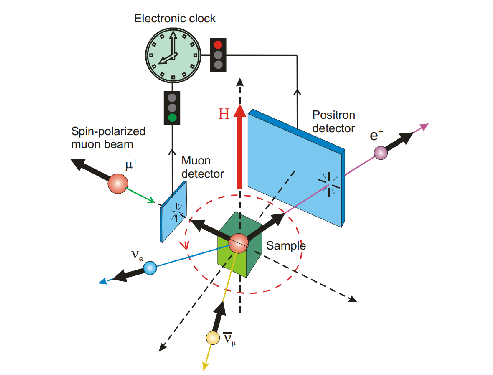
\includegraphics[width=0.65\linewidth]{spec.png}
\caption{Displays a simplified diagram of a conventional muon spectrometer found at TRIUMF.}
\label{spec}
\end{figure}
All current muon spectrometers employ the use of photomultiplier tubes (PMT's) for light detection. PMT's make use of the photo-electric effect and secondary emission for light detection. A schematic of one is shown in figure \ref{pmt}  . A photon incident on the device first collides into a photo-cathode screen where a primary electron is produce at an efficiency of about 1/4 (quantum efficiency). The primary electron is then accelerated through a focusing electrode onto the first dynode. Upon colliding with the surface secondary emissions occur releasing a burst of electrons. These are then again accelerated to another dynode again releasing more electrons during collision. This amplifying effect continues until the anode is reach for which the electrons are conducted out of the device as a electrical signal. The PMT effectively turns a single photon into millions of electrons enabling low light level detection. Because of the high bias used to power the dynodes the PMT produces a high signal to noise ratio, which makes them optimal for timing applications. However in a muon spectrometer PMT's can have many downsides. In addition to there high cost, PMT's can be cumbersome to work with.
\begin{figure}[h!]
\centering
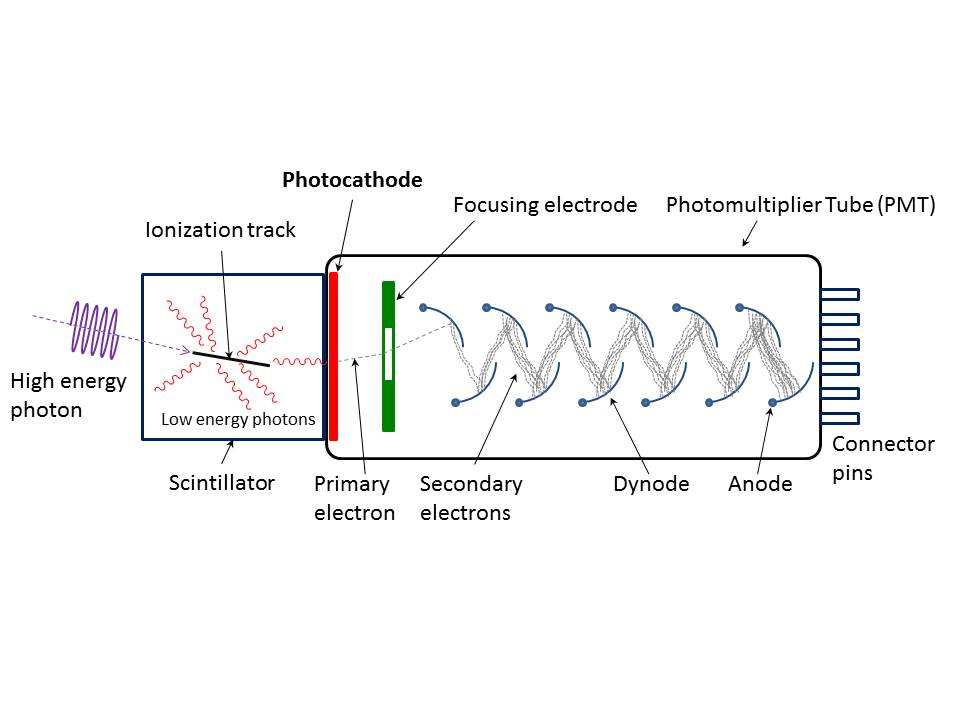
\includegraphics[width=0.65\linewidth]{pmt}
\caption{Displays a simplified diagram of a conventional photomultiplier tube (PMT).}
\label{pmt}
\end{figure} 
For example regular PMT's can not be exposed to a high magnetic field, and therefore special shielding is required in order to use them in the spectrometer. However the use of shielding can distort the magnetic field. In order to preserve the field and focused muon beam, placement of the PMT's requires symmetrical positioning and in some cases the addition long wave guides. This again limits spectrometer design and increases costs. These problems could potentially be solved with inexpensive silicon photomultiplier's.

\subsection{SiPM}
An avalanche photodiode (APD) is a sensitive semiconductor device that exploits the photoelectric effect to convert light to an electric signal.  APDs can be thought of as photodetectors that provide a gain through avalanche multiplication and can be considered as the semiconductor analog to photomultipliers. Figure \ref{adp}  displays a simplified diagram of the internal structure of a ADP. Silicon photomultipliers (SiPM's) are Silicon photon sensitive devices built from an array of APD's operating in Geiger mode. During avalanche breakdown when applying an external electric field to a semiconductor holes and electrons move to opposite ends. If the E field is high enough electrons can eject neighboring electrons, creating more holes and free electrons. The fast moving holes allow more e-hole pairs to form which means the crystal becomes conducting. In an Avalanche Diode the original carrier is created by the absorption of a photon. Once absorbed an electron is eventually ejected and in the presence of an external e-filed is accelerated which frees more electrons and holes. Newly ejected electrons also get accelerated which still have the ability to knock others free. The result is a shower of electrons and holes, resulting in measurable current, started by one photon. 

\begin{figure}[h!]
\centering
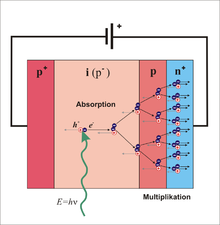
\includegraphics[width=0.30\linewidth]{adp.png}
\caption{Displays a simplified diagram of a conventional avalanche photodiode (APD).}
\label{adp}
\end{figure} 

The dimension of each single APD can vary from 20 to 100 micrometres. The supply voltage (Vb) depends on APD technology used, and typically varies between 20 V and 100 V, thus being from 15 to 75 times lower than the voltage required for a traditional photomultiplier tubes (PMTs) operatio. Photo detection efficiency (PDE) ranges from 20-50\% depending on device and wavelength. Gain of the device is also similar to a PMT being approximately $10^6$. The gain verse over-bias voltage dependence is linear, unlike PMT which follow the power law. SiPM signals are unaffected by external magnetic fields and because of their light, small design have little impact on the field itself. These are the key features which make SiPM's a viable option for future spectrometer design. 

\newpage
\section{Simulation}
\subsection{Introduction}
A large portion of work complete on this project involved simulating the effects and geometry and discrimination on timing. A simulation was written from scratch in c++, analyzed using ROOT and visualized using a simple openGL application. The simulation was designed to incorporate more geometric complex scintillation pieces. The architecture enables simulation of complex scintillation pieces. This portion describes the simulations in detail for future modification ability. For the purpose of clarity each single SiPM device will be referred to as a "pixel" while each pixel on the device will be referred to as "micro-pixels" (Sensl convention). The simulation with installation instructions for linux machines is available on my github: \textit{https://github.com/j16out/scintS}

\subsection{Program Layout}
 The simulation is divided into three essential scripts. The Upper layer most commonly referred to as the 'macro level' uses a subset of functions found in the two lower levels. The layout of the simulation run is defined in the upper macro layer. Although the simulation consists of approximately 8000 lines of code, the user only deals with 20-30, depending on their needs. Below describes the list of functions one would call in a typical run for a macro.
\begin{lstlisting}
//-----------loading model-------------//
    load_geometry(scintsurf, "Project1");//geometry
    load_sensors(sensorsurf, "Project1");//sensors

//-----------Generating Scintillation-------------//

    scintillation = getscintpath(scintsurf, 5000, 1.0, 1.0, 2.0, points, "Project1");

//-----------Propagating/Detecting Photons-------------//

    getphoton(AFpath, pathtime, scintsurf, sensorsurf, scintillation, sensindex);	     	

//-----------OpenGl visualization---------//

	Tanimate(AFpath);//reorganize for fancy animation
	res = cadpath(AFpath);//generate file for opengl

//-----------ROOT analysis-----------// 

	TApplication theApp("App", &argc, argv);
	SignalTime(pathtime, sensindex);
	visroot(scintillation,sensorsurf,scintsurf,AFpath,pathtime);
	theApp.Run();

//-----------End Sim-----------//

\end{lstlisting} 
The files gPT and mROOT are the two lower level includes. gPT contains are relevent simulation and mathematical functions. The mROOT files contain all functions related to histogram and signal analysis via ROOT.

\subsection{Creating Geometry and Sensors}
The main feature of this simulation is its ability to quickly import new geometry and sensors via .ast (STL) generated cad files. The geometry is created using any capable modeler. For a open-source parametric modeler FreeCAD was used, available for all platforms. The simulation will use the imported geometry as the reflective layer to accurately propagate photons internally through the piece. When designing geometry there are some things to consider. Speed is a huge factor, although the sim is multi-threaded, its speed is determined by the size of the imported geometry. More vertices means longer sim times. So avoid filleting edges unless absolutely necessary.

\begin{figure}[h!]
\centering
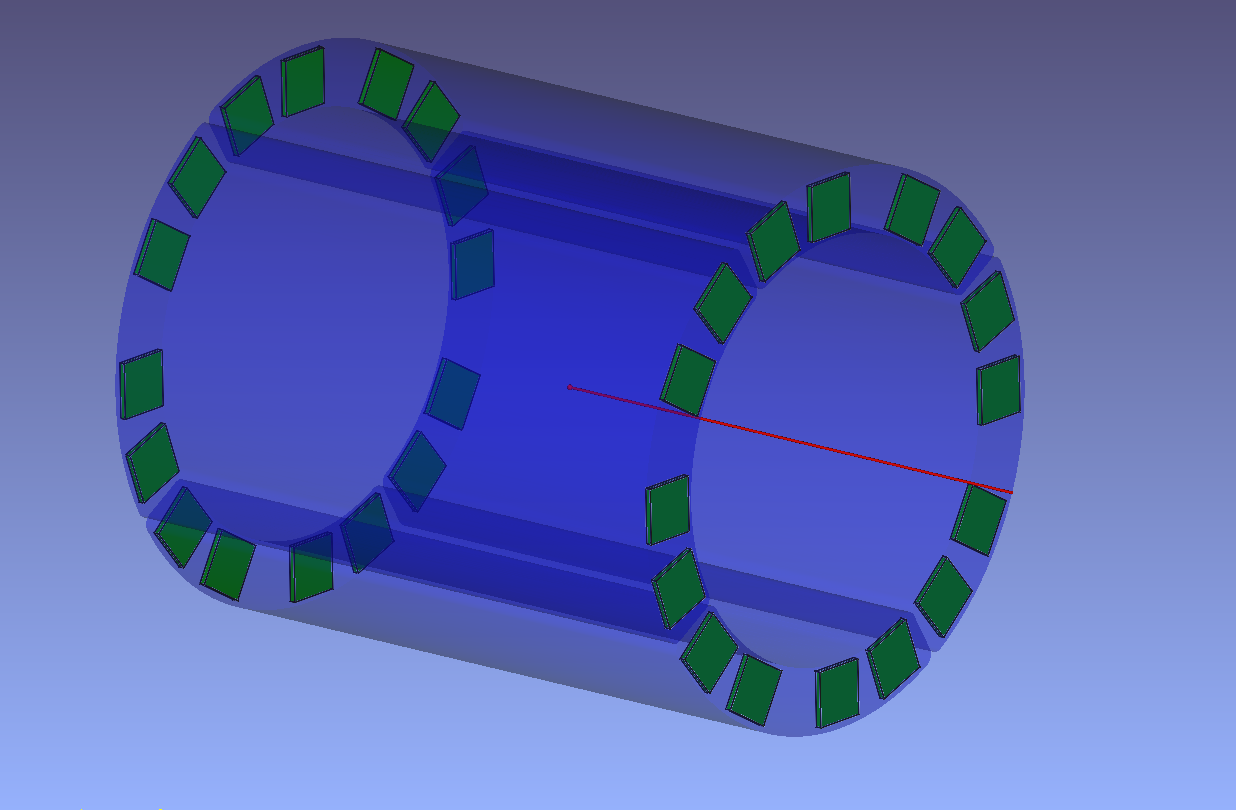
\includegraphics[width=0.70\linewidth]{fcad}
\caption{Displays an example of geometry (clear blue) and sensors (green) created using freecad.}
\label{geosens}
\end{figure}

 When generating mesh, be mindful of what density of vertices is required for your application. Obviously a higher density mesh will be more realistic and provide better accuracy as it more accurately represents a curved surface, however its at the expense of longer simulation times. The simulation requires two imports, one for geometry and the other for sensors. Sensors are imported the same way the geometry is using the
 \begin{verbatim}
  load_geometry("3D vector", "Project Directory")
  load_sensors(3D vector", "Project Directory") 
 \end{verbatim} 

 functions provided by gPT includes. The load functions require a 3D vector and the path of the project directory.The 3D vector will be filled with the vertice information from both the sensors and geometry. Figure \ref{geosens} displays an example of a geometry/sensor (G/S) set created using freeCAD. The simulation requires a ascii stereo-lithography file denoted '.ast' which contains all vertice and facet data. The simulation will use this data to build boundaries that will affect propagating photons.  The simulation requires a 'Project' folder which needs a specific layout. A directory for geometry and sensors are required. Geometry and Sensor .ast files are required to be labeled as g1 and s1 respectively. For designs requiring multiple G/S's models are to be named in succession and placed in the G/S directories. Ie A design with 4 sensors will require a sensor directory with 4 models labeled s1, s2, s3 and s4. When the simulation uploads the sensors an index will be generated keeping track of which detectors are stimulated. If one wishes to sum 4 sensors they should all be exported in the same .ast files ie only one sensor file (s1).
 

\subsection{Positron Generation}
Once geometry and sensors are imported into the simulation, the starting points of the photons need to be generated, ie positron generation. Start points are randomly produced along a trajectory set by the positron generator function. In addition random directions for photon propagation are also generated in this step. all are stored for later use in a 2D vector. For visualization the trajectory is used to manipulate a 'positron path' model used in the openGL visualization. The is all accomplished by retrieving the randomly generated data via the 
\begin{verbatim}
  getscintpath()
  getlaserpulse()
 \end{verbatim} 
functions, One for scintillation signal and laser signal respectively. When setting a positron or laser pulse trajectory its imperative to ensure it intercepts a scintillation piece. The path is able to intercept multiple pieces without any problem as displayed in figure \ref{multscint}, however its imperative the positron begin outside of the geometry, as it uses a primitive indexing system to know whens its inside or outside the scintillation piece ie its needs to intercept two surfaces to register a single scintillator piece. So if the positron begins inside the scintillator the simulator will only see it intercept one surface, and therefore will not register as a scintillating event and subsequently an error will occur. 

\begin{figure}[h!]
\centering
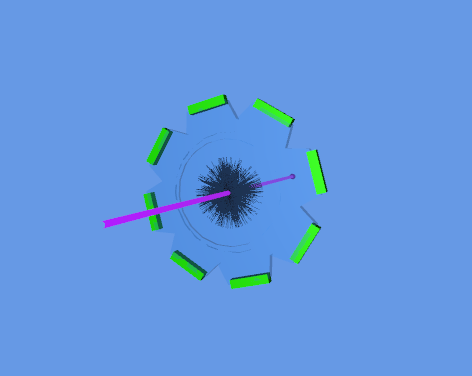
\includegraphics[width=0.70\linewidth]{posi2.png}
\caption{Displays simulated photon paths (black traces) originating from positron path (purple) and propagating to sensor (green).}
\label{simpic}
\end{figure}

\begin{figure}[h!]
\centering
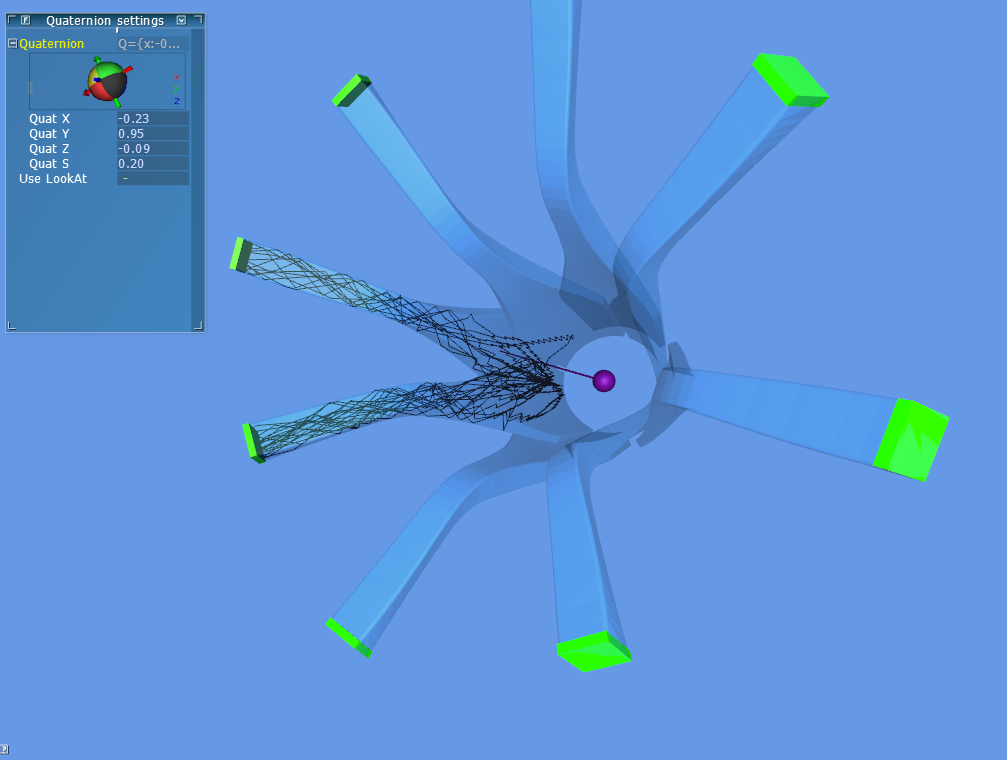
\includegraphics[width=0.70\linewidth]{posi3.png}
\caption{Displays the programs ability to simulate complex scintillation structures.}
\label{simpic}
\end{figure}

\begin{figure}[h!]
\centering
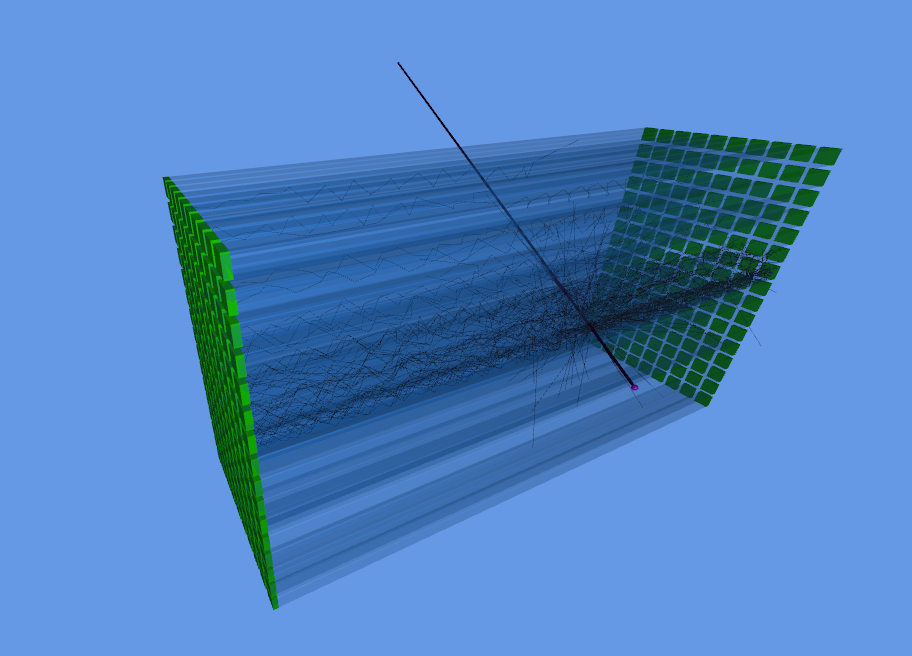
\includegraphics[width=0.70\linewidth]{multscint.png}
\caption{Displays the multiple intercept capabilities of the simulator. Positron intercepts multiple pieces producing scintillating photons in each.}
\label{multscint}
\end{figure}

\subsection{Photon Propagation}
Photons are permitted to propagate from the point of origin until a boundary is reached. The scintillator boundary is defined by cluster of interlocking triangles, ie a mesh. If the photon intersects the boundary then it must intercept one of these triangles that make up the surface. The simulator imports the .ast mesh file and builds a vector of triangles which makes up the surface. Once a photons random direction is selected, an algorithm is used to check to see if it intercepts any of the triangles along its path of flight. If an intersection is detected, a intercept point, and reflected vector are calculated and the simulation begins rechecking for triangle intercepts using the new reflected direction. This process yields the path of the photon and subsequently the time of flight as it propagates through the scintillation piece. 

The Algorithm employed is nearly identical to the Ray and triangle intersection computation that is used in computer graphics rendering programs. Assume we have a ray $R$ going from points $P_0$ to $P_1$, and a plane P through $V_0$ with normal $n$. The parametric line $L$ denoted as $P(r)=P_0+r(P_1-P_0)$ and intersects the plane $P$ at the point $P(r_I)$ with parameter value:


\begin{equation}
\label{rI}
r_I=\frac{n\cdot(V_0-P_0)}{n\cdot(P_1-P_0)}
\end{equation}

When the denominator $n\cdot(P1-P0)=0$, the line $L$ is parallel to the plane $P$ , and thus either does not intersect it or else lies completely in the plane (whenever either P0 or P1 is in P ). Otherwise, when the denominator is nonzero and $r_I$ is a real number, then the ray $R$ intersects the plane P only when $r_I\geq0$. A segment S intersects P only if $r_I\geq0\leq1$. In all algorithms, the additional test $r_I\leq1$ is the only difference for a segment instead of a ray.
Intersection of a Ray/Segment with a Triangle

Consider a ray R from $P_0$ to $P_1$, and a triangle T with vertices $V_0$, $V_1$ and $V_2$. The triangle $T$ lies in the plane $P$  through $V_0$ with normal vector $n=(V_1-V_0)\times(V_2-V_0)$. To get the intersection of R with T, one first determines the intersection of R and P . If it does not intersect, then it also does not intersect T and we are done. However, if they intersect in the point $PI = P(rI)$, we need to determine if this point is inside the triangle T for there to be a valid intersection.

 The parametric plane equation is given by:
 
 \begin{equation}
\label{vsl}
V(s,t) = V_0+s(V_1-V_0)+t(V_2-V_0) = V_0+su+tv
\end{equation}

where $u=V_1-V_0$ and $v=V_2-V_0$ are edge vectors of T. Then, $P=V(s,t)$ is in the triangle T when $s\geq0$, $t\geq0$, and $s+t\leq1$. So, given $P_I$, one just has to find the $(s_I, t_I)$ coordinate for it, and then check these inequalities to verify inclusion in T. Further, $P=V(s,t)$ is on an edge of T if one of the conditions $s = 0$, $t = 0$, or $s + t = 1$ is true (each condition corresponds to one edge). And, the three vertices are given by: $V_0=V(0,0)$, $V_1=V(1,0)$, and $V_2=V(0,1)$.

\begin{figure}[h!]
\centering
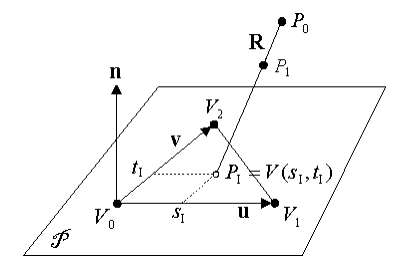
\includegraphics[width=0.5 
\linewidth]{alg.png}
\label{alg}
\end{figure}

There all that is left is to find $s_I$ and $t_I$.  With $w=P_I-V_0$, which is a vector in P  (that is, $n\cdot(w)=0$), we solve the equation: $w=s_u+t_v$ for s and t. The final result is:

 \begin{equation}
\label{fs}
s_I= \frac{(u\cdot v)(w\cdot v)-(v\cdot v)(w\cdot u) }{(u\cdot v)^2-(u\cdot u)(v\cdot v)}
\end{equation}

 \begin{equation}
\label{ft}
t_I= \frac{(u\cdot v)(w\cdot u)-(u\cdot u)(w\cdot v) }{(u\cdot v)^2-(u\cdot u)(v\cdot v)}
\end{equation}

which has only 5 distinct dot products. It has been arranged in terms so that the two denominators are the same and only need to be calculated once.

When the geometry and Sensors are loaded and a positron path has been defined photon propagation can be iterated. Using the algorithm described above photon travel times are calculated from start until its reaches a sensor. Photons that encounter boundaries at angle below the critical angle (relative to normal) will transmit out of the scintillator, these photons are stopped and times are discarded. If the 'RT' code is used a transmitted path will be loaded into the openGL visualizer (default). Reverting to 'R' code will only display internally reflected photons. Photons that arrive at the sensor surface at angle greater than critical angle (relative to normal) are also discarded as the photon would not transmit into the detector. The critical angle can be adjusted inside the gen() function called by the multi-threading method getphoton().



\subsection{Final Signal}
In addition to providing the distribution of arrival times the final signal from each sensor is calculated. This is done by summing all the individual micro-pixel signals with the timing adjustment, which is denoted as $t_o$ in equation \ref{risefall}.



\begin{equation}
\label{risefall}
V(t) = V_{max} (exp(\frac{-(t-t_{o})}{\tau_{Rise}})-exp(\frac{-(t-t_{o})}{\tau_{Fall}}))
\end{equation}

The program applies each timing adjustment before summing all the signals. The signals are summed and stored in a vector. The size of the vector denotes the resolution of the signal, ie each component of the vector represents a point in the final function. Initially the entire vector is set to zero. Then the timing adjustment is imputed into a function which is then evaluated for each component in the vector. The process continues for each timing adjustment as shown below.

\begin{lstlisting}
for(int n = 0; n < ftime.size(); ++n)
	{
	for(int i = 0; i < graphs1A.size(); ++i)
		{
			tomp = -(11.94)*(exp(-((i*.001)-ftime.at(n))/2.341)-exp(-((i*.001)-ftime.at(n))/9.526));
			if (tomp > 0)
			{
				if(Sfinpos1.at(n) == 1)
				graphs1A.at(i) = tomp + graphs1A.at(i);
				if(Sfinpos1.at(n) == 2)
				graphs1B.at(i) = tomp + graphs1B.at(i);
				if(Sfinpos1.at(n) == 3)
				graphs1C.at(i) = tomp + graphs1C.at(i);
				if(Sfinpos1.at(n) == 4)
				graphs1D.at(i) = tomp + graphs1D.at(i);
			}
			else
			{
				if(Sfinpos1.at(n) == 1)
				graphs1A.at(i) = 0 + graphs1A.at(i);
				if(Sfinpos1.at(n) == 2)
				graphs1B.at(i) = 0 + graphs1B.at(i);
				if(Sfinpos1.at(n) == 3)
				graphs1C.at(i) = 0 + graphs1C.at(i);
				if(Sfinpos1.at(n) == 4)
				graphs1D.at(i) = 0 + graphs1D.at(i);
			
			}
		}
}
\end{lstlisting}

 This makes for an efficient and memory saving method for calculating the final function. There are a couple of lines which organize all timings into specific groups corresponding to different pixels. These final signals are then shifted based on a threshold, then the intercept is calculated. This gives the timing of the applied threshold. These are saved from each signal then checked for coincidence. If all signals from each pixel are above threshold, then the earliest time is stored. If one signal is not above threshold the entire run is discarded. The earliest signal from each end of the scintillator is then saved and used for statistics. The simulation will then reset for another event. The results of all the events are tallied and used to determine the timing resolution of the experiment. figure \ref{simd1}  is an example of the final output for the simulation. In addition to the final data being saved in '.root' files, a log of the simulation is stored in '.txt' for future analysis or debugging.

 
 \begin{figure}[H]
\centering
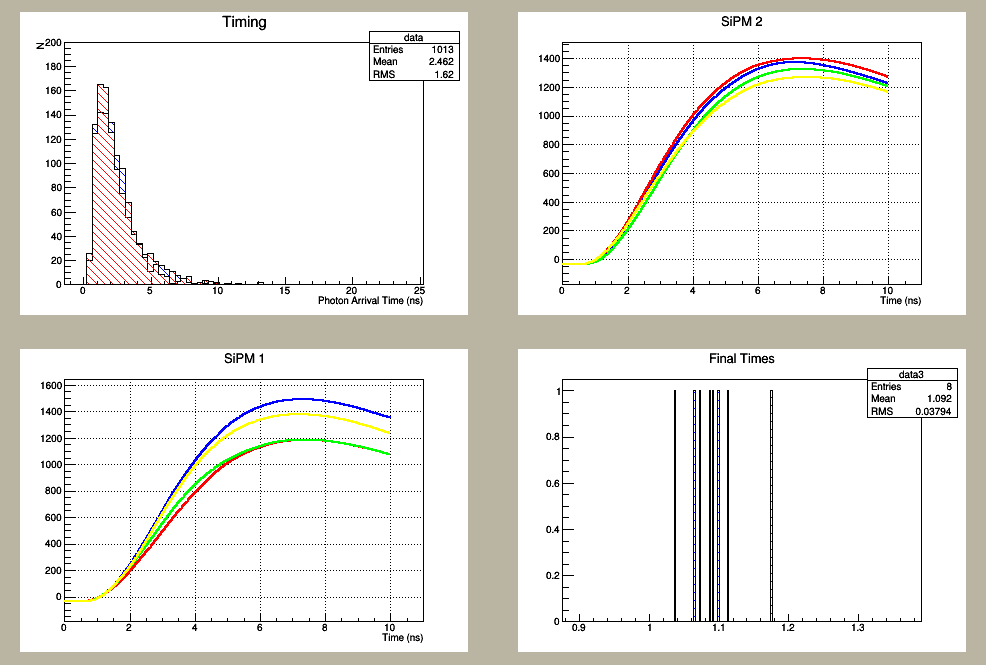
\includegraphics[width=0.80\linewidth]{simd1}
\caption{Displays a sample output of the simulator. The first graph shows all timings, the 2nd and 3rd show the final signals from each array, while the last shows the results of threshold timing.}
\label{simd1}
\end{figure} 
\newpage
\newpage
\newpage
\section{Oscilloscope Data Acquisition}

A large portion of the semester was spent on data acquisition and signal analysis. The final electronics design will exclude waveform data, therefore a simple waveform acquisition script was the appropriate choice. Basic communication scripts for the tds7104 were provided by Steve D. Sharples. The repository can be found at https://github.com/applied-optics/vxi11. The scripts were modified and tailored to fit the needs of the project. This section describes how to use the new scripts for various acquisitions. These scripts have been successfully tested in Scientific Linux and Ubuntu 14.04LTS and should work in other versions.


\subsection{Basic Operation}
To run the new scripts simply download and compile the file provided (tekvisascript.zip). Navigate to the directory containing the zip file and unload in any directory one desires. Then use the terminal commands provided:

\begin{verbatim}


  $ unzip tekvisascript.zip
  $ cd tek_1.04/
  $ make
  
  \end{verbatim}

If this compiles correctly and without any warning one can begin taking traces. To take data navigate to the $/tgetwf$ directory and run the following commands
\begin{verbatim}
 $ cd utils/tgetwf/
  
$ ./tgetwf -ip (ip adress of scope) -f (filename) -c (channel) -r (number of traces you want to acquire)
\end{verbatim}
heres an example for clarity:

\begin{verbatim}
$ ./tgetwf -ip 142.90.104.79 -f Laz_120PE_26.5V -c 2 -r 1000
\end{verbatim}



This should generates two files, .wf and .wfi which will be located in the $/tgetwf$ directory by default. The '.wf' is the data binary file and '.wfi' is the information file which contains scaling and offset values needed to interpret the binary data correctly. Here are some additional notes to consider when taking data which these scripts: If you clip the waveform (vertical) in the trace NO data will be recorded/sent for that part, this will be important to consider if one wishes to preserve linear timing data. Included also is the (vxi11/) you can use this for sending individual commands to scope ie taking/sending measurements adjusting scope acquisition parameters etc...Instructions on how to set this up are in the scripts.


\subsection{Binary Conversion}
First run trace graber(./tgetwf -ip your.ip.adress -f filename -c channel -r numruns), provided and as described above. Next convert binary file (.wf) to hex using unix/linux commmand: 
\begin{verbatim}

$ hexdump -x < binaryfile.wf > hextextfile.txt

\end{verbatim}
This command makes a file full of strings which can be sorted and converted into a float value. Each line should follow this format below, if it doesn't this string sorter won't work and need to make appropriate adjustments (DPO 7000 series was different)

\begin{verbatim}
0000000    4f00    5000    5100    5100    5300    5400    5100    5000
0000010    5100    5200    5300    5100    5000    5200    5000    5100
0000020    4f00    4f00    5000    4d00    5000    4e00    4f00    4d00
0000030    4f00    4f00    4d00    4d00    4f00    4d00    4c00    4e00
\end{verbatim}


Each line should be 71 characters long, if not it will be dismissed, sometimes a line is emty or filled with garbage. The vxi-11/tekVISA binary transfer protocol is 2 byte 8 bit signed.
These are formatted into a vector like this (first line from above):
\begin{verbatim}
 4f    50    51    51    53    54    51    50
\end{verbatim}


Each value in the string is then converted to 8 bit signed integers, then converted to floats and adjusted based on parameters from the .wfi file provided by trace grabber like this. There are simpler methods that can be explored that would hopefully avoid using the hexdump command and import directly from the binary file.
\begin{lstlisting}
for(int i = 0; i < hex.size(); ++i)
                {temp = hex.at(i);
                unsigned long int x;  
                 std::stringstream ss;
                        ss << std::hex << temp;
                        ss >> x;
                int y = (int8_t) x;
                float f = ((256*y*vertgain)-vertoff)*1000;//into mV
                // output it as a signed type
                        fin.push_back(f);
                //cout << "\n" << f;//for debugging
                }

\end{lstlisting}
\subsection{Laser/Power Supply Automation}
Both the Laser Attenuation and Power Supply employ a serial port for external communication. A simple serial communication script was created to change the setting during acquisition. It acts as the upper level, calling on the 'tgetwf' executable after adjusting the settings. The parameters of each waveform grab can be adjusted within the system() call of the program as display below:
\begin{lstlisting}
int main()
{
  int i=0,
      cport_nr=0,        /* /dev/ttyS0 (COM1 on windows) */
      bdrate=9600;
      
      float run = 12;  
       const char * c;
       string wave;
       string lasdb;
       int db = 40;
  for(int q = 0; q < run; ++q)
  {	  
  	wave = "./tgetwf -ip 142.90.99.12 -f file_db";
  	lasdb = "A";
  	db = q+18;
  	wave.append(tostr(db));
  	wave.append(" -c 1 -r 10");  	
  	lasdb.append(tostr(db));
  	lasdb.append("\r");
  	c = lasdb.c_str();
	  strcpy(str[0], c);
	  if(RS232_OpenComport(cport_nr, bdrate, mode))
	  {
	    printf("Can not open comport\n");
	    return(0);
	  }
	    RS232_cputs(cport_nr, str[i]);
	    printf("sent: %s\n", str[i]);
	    cout << "\n changing laser attenuation";	    
	    usleep(4000000);	    
	    c = wave.c_str();
	    system(c);    
    }
return 1;
}
\end{lstlisting}
The script consists of a 'string appender' which builds the 'tgetwf' command with proper arguments, it is then executed with the system() command. The script will wait until run is complete before continuing. The usleep() is used to allow proper time for the attenuation to adjust before starting acquire. The string lasdb is the ascii command sent to the attenuation via serial port. If left unattended one should set a high attenuation before program terminates too avoid over exposing SiPMs. This can be used in other serial applications, one just needs insert appropriate serial commands. Serial Communication is available via different baud rates and ports, see rs232.c for appropriate settings. 
\newpage
\section{VME/MIDAS Data Acquisition}
\subsection{Overview}
"MIDAS" is an acronym for Maximum Integrated Data Acquisition System and is a general-purpose software package for event-based data acquisition in small and medium scale Physics experiments. A VME/MIDAS crate has been setup as the main data acquisition system for the final spectrometer. The VME hardware consists of a computing card, TDC, QDC, clock and constant fraction cards. The PCM computing card is used to run the frontend program in midas. Its task is to communicated and retrieve data from the cards in the crate and prepare data for transfer to remote or local clients. The main server and the PCM card run the midas client and server services. Since the documentation is extensive and well written by the MIDAS collaboration, only the parts that were modified will be discussed in this document. More detailed information about MIDAS setup and operation can be found here:
\newline
$https://midas.triumf.ca/MidasWiki/index.php/Midas_documentation$
\newline
 
\begin{figure}[h!]
\centering
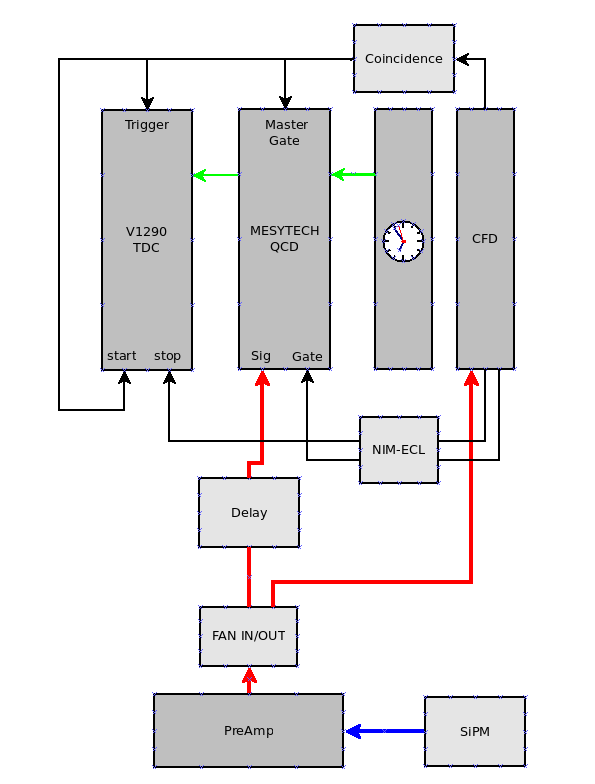
\includegraphics[width=0.70\linewidth]{schem1.png}
\caption{A schematic of the VME interface}
\label{cs}
\end{figure}

\subsection{Starting VME Acquisition}
During my time at triumf the data acquisition system was run on the \textit{daq01} computer provided by the data acquisition group. The user account for which the midas server can be launch was \textit{musr\_ 3t}. As I was not given access to this account I would simply ssh in from an account for which I had added accepted keys. In this case the \textit{mppc@daq01} account has such access. The password for this account is \textit{'muione\_ 2014'}. Once logged into this account I would ssh into \textit{musr\_ 3t} using following command.
\newline
\newline
\textit{ssh -vX musr\_ 3t@daq01} 
\newline
\newline
The -v gives information about the login 
while the -X enables X11 forwarding operations which is crucial for opening the Midas analyzer remotely. Once logged in the server can be started. move to the \textit{~/online/bin/} directory. This should contain the startup executable which can be run using  \textit{./start\_ daq} command. Once this is started we can now launch the secure mhttpd server which will host a panel for controlling the experiment. The MIDAS web server mhttpd is explicitly linked with OpenSSL to provide secure HTTPS connections via the Mongoose web server. To start the web server in the background simple enter this command.
\newline
\newline
\textit{mhttpd -D -p(prefered port)}
\newline 
\newline
If a port option is not enter it will start on default secure 8443. Now to access the experimental control panel enter the address into a web browser.
\textit{https://myhost.mydomain:8443}
It will prompt for username and password. If one needs to create a new username or password see the MIDAS documentation here:
 \textit{https://midas.triumf.ca/MidasWiki/index.php/Mhttpd}
Once your credentials are accepted you should be redirected to the midas control panel. This provides a GUI interface for controlling the analyzer, front-end, MSCB and other functions featured in Midas. To run a data collection run or an experiment one needs to start the front end, this can be done either manually or via the web server. For manual start one will need to ssh into the control card on the VME crate labeled \textit{lxdaq24} from the \textit{musr\_ 3t} account. Once logged in move to the \textit{/online/src/} directory which should contain the fe3t executable. Running this will start the front end. Also found in this directory is the main script \textit{fe3t.cxx} for front end operations. This script configures each card in the crate at start up, and contains some lines for card communication and manually setting registers. An example is the \textit{mesqdc32\_ RegisterWrite()} function which was use to set the configurable options for the mesytek such as termination, thresholds and gate modes. The register information and variables can be found in \textit{OdbMesqdc32.h mvmestd.h} driver files. Once the front end has initiated and is running on the lxdaq24 system, the analyzer can be started from any machine with acceptable credentials. 

\subsection{ROOTana Analyzer}
Like the front-end it can be started both manually or through the mongoose web server. To start manually log into the \textit{musr\_ 3t@daq01} account. Move into the \textit{~/nana3t/src/} directory which contains all the source and executable for running the analyzer labeled \textit{./anaDisplay} executing this will launch a display window which will begin displaying real time data for the current run.  Once the analyzer is launched one can begin collecting data by starting the run through the mongoose web server. The window contains tabs for each type of data set being acquired, as well as controls fro defining refresh rates and which channels to view. New tabs or data set can easily be added by creating new appropriate objects. In our case a data set displaying both charge (mesytech) and time (v1290) was required. I went forth and created a new object called \textit{T2DHistogram.o} by adding appropriate lines in the makefile, \textit{TAnaManager.cxx} and \textit{TAnaManager.hxx} files. I then built a set of functions for adding data into the object described in the \textit{T2DHistogram.cxx} file. This script for each run pulls data from the TDC and QDC, event matches, then plots charge vs time in a 2D histogram for a particular channel as shown below. Similarly the \textit{V1290HistogramdTime.cxx} script histograms the registered TDC hits of channels 1-15 relative to a reference sent to channel 0 while the \textit{MQDCHistogram.cxx} histograms the level of charge measured in channels 1-16. To save the data collected as a root file, pause the analyzer and stop the run using the midas mongoose web-page. ROOT files are stored in the \textit{~/nana3t/src/} directory where the analyzer was launched.

\subsection{T2DHistogram Breakdown}
Here is a simple breakdown of the T2DHistogram.cxx script and how it can be used to take automated measurements. The script contains the functions CreateHistograms(), UpdateHistograms(), BeginRun() and, EndRun(). The BeginRun() function runs before data collection begins starting the laser, power supply and histogram creation. The 2D and 1D histograms are created in the CreateHistograms() function via the following lines:
\begin{lstlisting}
for(int i = 0; i < 3; i++){ // loop over channels    
    char name[100];
    char title[100];
    sprintf(name,"MesQDC_%i_%i",0,i);
     // Delete old histograms, if we already have them
    TH2D *old = (TH2D*)gDirectory->Get(name);
    if (old){
      delete old;
    }
    // Create new histograms    
    sprintf(title,"Sum of Sides channel=%i",i);	    
    TH2D *tmp = new TH2D(name,title,1000,-50,50,2000,-2000,2000);
    tmp->SetXTitle("TDC value");
    tmp->SetYTitle("QDC value");
    tmp->SetOption("colz");
    push_back(tmp);
}
\end{lstlisting}
It loops over all the channels creating a histogram for each (in this case its limited to 4 channels) and setting the appropriate boundaries and number of bins. If one wants to add anything else to the root histograms this is the place to add lines, like setting the style, color, title etc.
Once the histograms are created they are updated every n events, where n is set in the analyzer display. The UpdateHistograms() contains the lines responsible for filling the histograms with data aquired from the midas server. In Midas the data is held in globaly in memory and can be extracted into an object vector created using the GetMeasurements() function. The QDCmeasurement and TDCmeasurement vectors contain both the data, run info and channel data. These can be extracted by the GetChannel() and GetMeasurement() functions as shown below.

\begin{lstlisting}

// Get the Vector of ADC Measurements.
  std::vector<QDCMeasurement> measurements = data->GetMeasurements();
  std::vector<TDCMeasurement> Tmeasurements = Tdata->GetMeasurements();
  
  std::vector<float> QDCfdata;
  std::vector<int> indexQDCfdata;
  std::vector<float> TDCfdata;  
  std::vector<int> indexTDCfdata;
  
//For QDC
  for(unsigned int i = 0; i < measurements.size(); i++){ 
    int chan = measurements[i].GetChannel();
    QDCfdata.push_back(measurements[i].GetMeasurement());
    indexQDCfdata.push_back(chan);
  }
//For TDC notice reference value stored differently
   for(unsigned int i = 0; i < Tmeasurements.size(); i++){ 	
    int chan = Tmeasurements[i].GetChannel();
    if (chan == 0) {  
      tRef2 = Tmeasurements[i].GetMeasurement();
    } else {
      tempval2 = Tmeasurements[i].GetMeasurement();
      TDCfdata.push_back(tempval2);
      indexTDCfdata.push_back(chan);
      std::cout << " ch[" << chan << "]=" << tempval2;
    }
  }
\end{lstlisting}

Now both the channel number and data have been extracted into vectors. Due to the structure of the Midas system, data doesn't arrive sequentially relative to channel number, therefore to match channels between the QDC and TDC, the data needs to be reorganized according to channel as shown below. The \textit{if} statement is used for coincidence to ensure data is being plotted only if both the QDC and TDC have hits on a particular run. In this case we are expecting data on 2 channels for both QDC and TDC.

\begin{lstlisting} 
std::vector<float> QDCfinaldata (measurements.size());
std::vector<float> TDCfinaldata (Tmeasurements.size());

if(TDCfdata.size() == 2 && QDCfdata.size() == 2)
{
	for(unsigned int i = 0; i < QDCfdata.size(); i++)
	{
	int chan = indexQDCfdata.at(i);
	if(chan <= QDCfdata.size())
		QDCfinaldata.at(chan) = QDCfdata.at(i);
	}

	for(unsigned int i = 0; i < TDCfdata.size(); i++)
	{
	int chan = indexTDCfdata.at(i);
	if(chan <= TDCfdata.size())
	    TDCfinaldata.at(chan-1) = TDCfdata.at(i);
	}
}
\end{lstlisting}
Now that the data has been reorganized it can be stored into a histogram using the GetHistogram() and Fill() functions. The process for both 1D and 2D histograms is the same and only differ in the number of variables required by the fill function. It is at this point a curve correction can be applied as well. Below the uncorrected data is stored in the first two histograms while the corrected data is stored in 3rd and 4th.

\begin{lstlisting}
if(TDCfdata.size() == 2 && QDCfdata.size() == 2)
{	
    for(unsigned int i = 0; i < 2; i++)
	{
	    float data1 = QDCfinaldata.at(i);	
	    float data2 = (TDCfinaldata.at(i)-tRef2) * 0.025;

		fcount = GetHistogram(i)->GetEntries();
		if(atten <= 26 && fcount <= fcount2)	
		  {float pp0, pp1, pp2;
		  GetHistogram(i)->Fill((data2), (data1));
		  //curve correction 
		    float dataC;
			float pp0 = 10900, pp1 = 0, pp2 = -5138;//curve correction pars
			dataC = data2 -((sqrt(pp0)/sqrt(data1-pp2))+pp1);
			GetHistogram(i+2)->Fill((dataC), (data1));
		  }	      
	}
}	
\end{lstlisting}

The \textit{UpdateHistograms()} function also contains a couple of lines for controlling the laser. When the histograms are filled they are also checked for content using the \textit{GetEntries()} function which is used by the laser control. In the case below the laser was required to change every 10000 entries, \textit{fcount} being the current number of entries and \textit{fcount2} being the target level. Once reached the script uses a system command to run an external RS232 communication program called in this case \textit{Go} which requires a single argument; attenuation level. A pause is implemented to ensure the attenuation has time to change before midas continues acquisition 
\begin{lstlisting}
if(fcount > fcount2 && (atten <= 26))
	{
	 atten = atten + 0.1;
	 std::cout  << "\n count:  " << fcount;
	 const char * c;
	 std::string com1 = "/home/musr_3t/bin/Go -d ";
	 com1.append(tostr(atten));
	 c = com1.c_str();
	 system(c);
	 fcount2 = fcount2 + 10000;        
	 usleep(2000000);
	}
\end{lstlisting}

The Laser Control Program is located in the simpData folder on the musr OneDrive under Jerin Roberts work and also in the compressed folder sent with this report. In the appendix is an overview of the laser control program, the executable is created using g++ and requires the rs232.c/h scripts (onedrive). The program consists of a string appender which generates an ASCII command which is then written to the rs232 compatible port, in this case we used a usb to rs232, henceforth the \textit{/dev/ttyUSB0}. The string appender can be reconfigured to send any command therefore this can be used for any rs232 control, ie power supply automation. 
\newpage  
\section{Dectector Tests}
The electronic detector group was asked to design the front end electronics for the spectrometer, which required characterization of the devices of choice. One SiPM from sensl was selected as the most viable option. Figure \ref{cs} shows the devices used and tested. At the time the low noise C-series 6mm device hadn't been released. In order to advance electronics design earlier models were characterized. Both the 3mm B-series and 6mm C series (non-lownoise) were characterized.
\begin{figure}[h!]
\centering
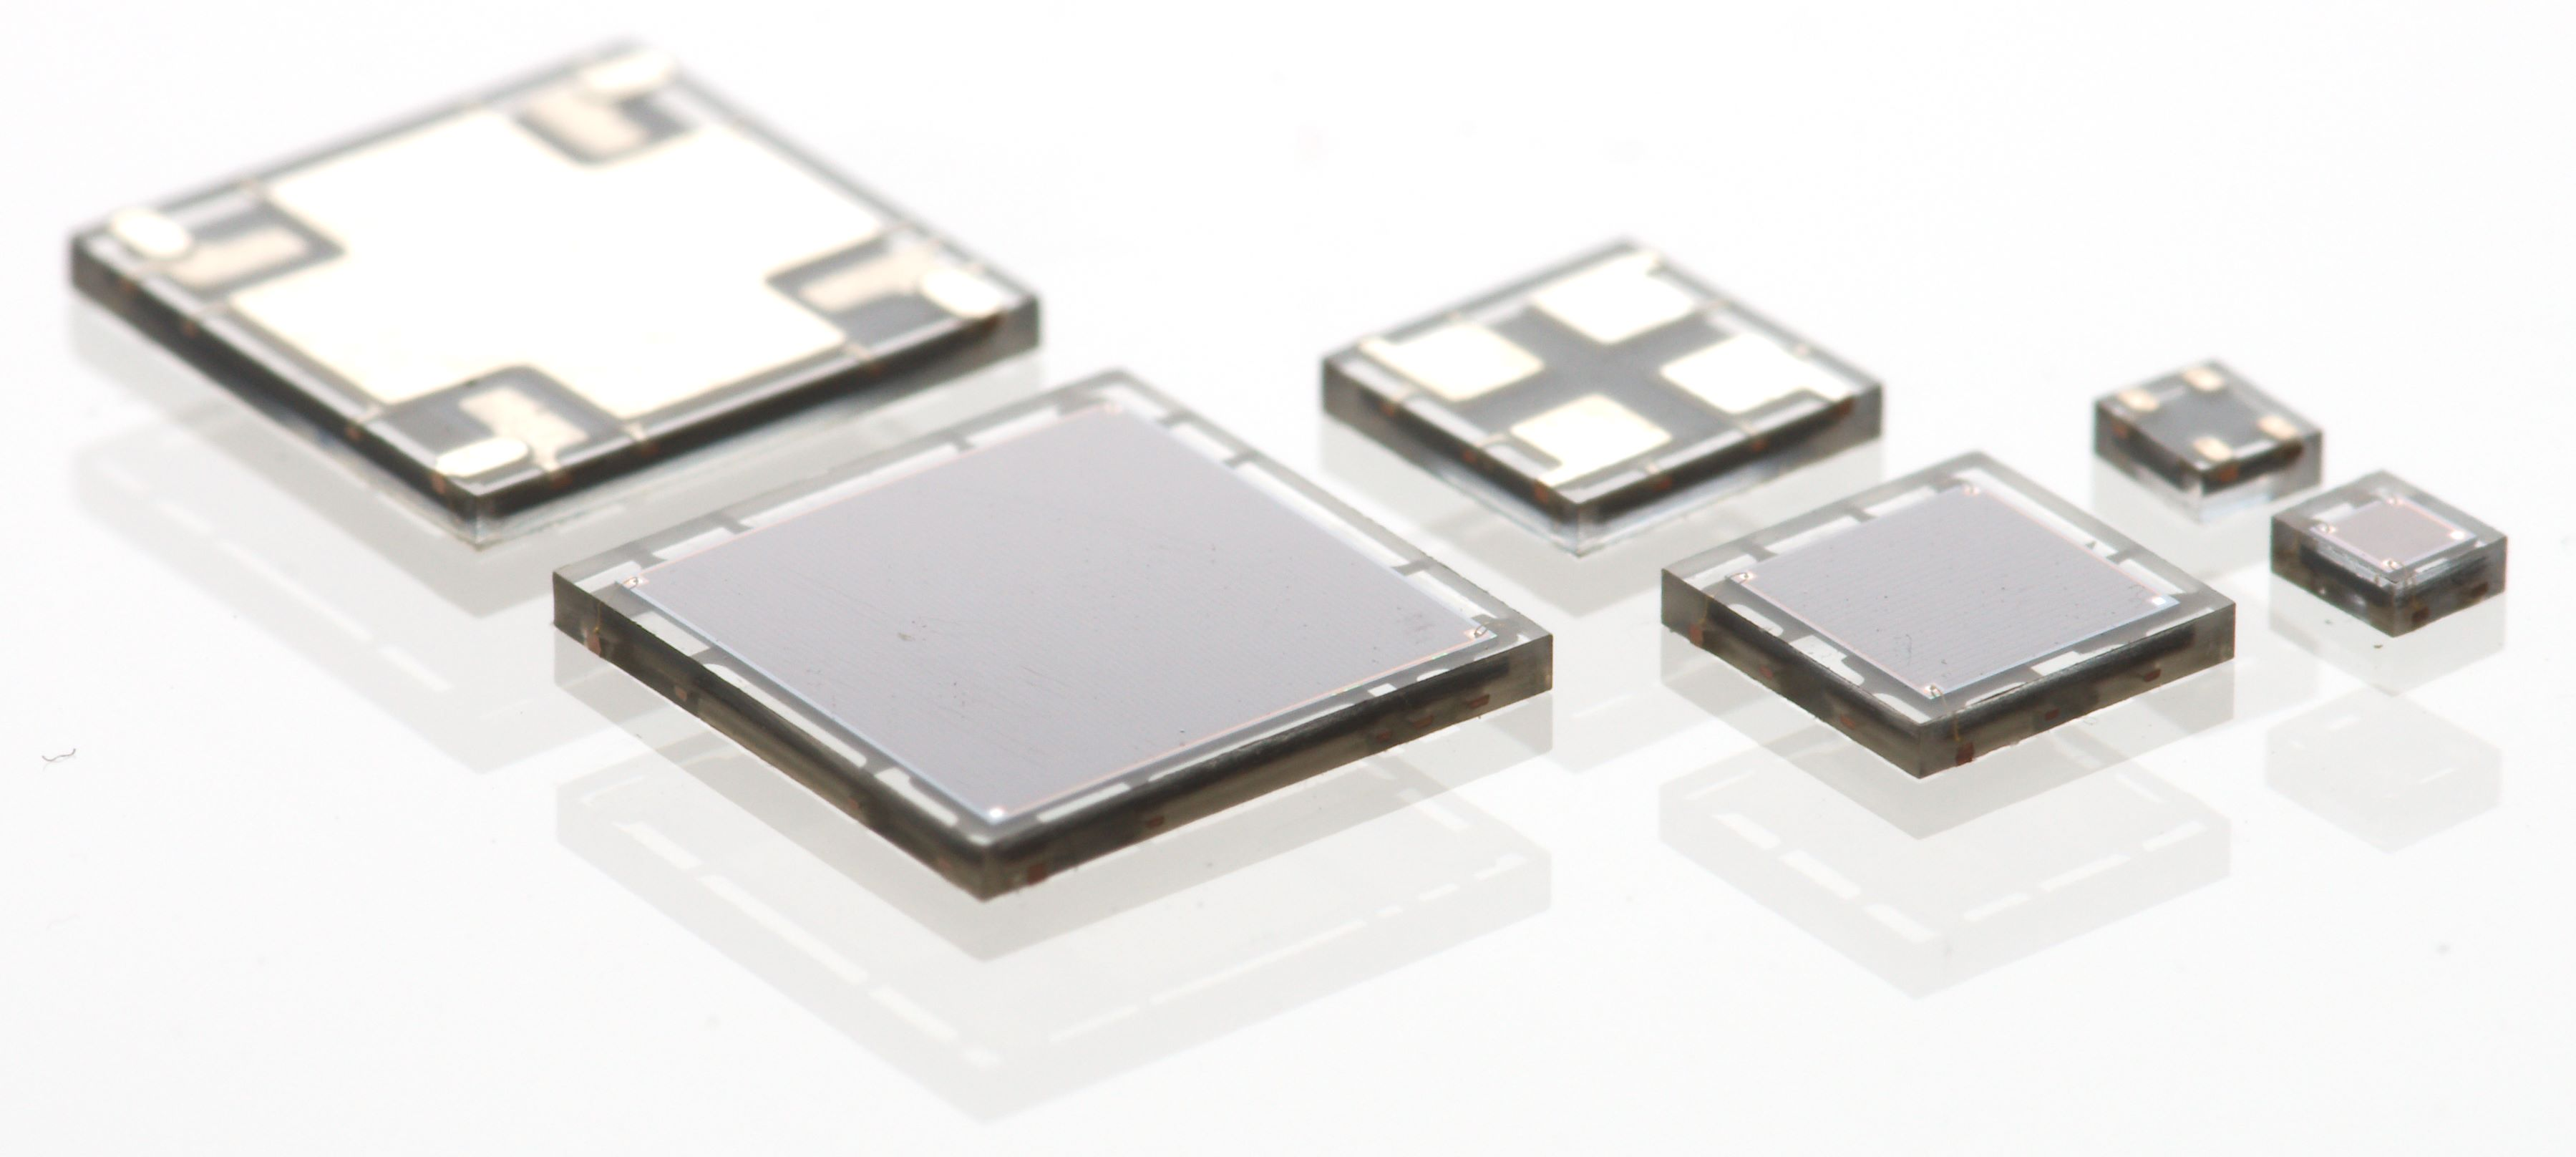
\includegraphics[width=0.70\linewidth]{cs}
\caption{A picture of the devices used for detector tests; 6mm c-series and 3mm b-series.}
\label{cs}
\end{figure}
    
\subsection{Apparatus Design}
In order to perform detector tests a custom apparatus needed to be designed and fabricated. A slotted bracket and breadboard style design was selected for its adjustability and adaptability for different tests while a light and EMI tight box was built to lower noise. Each piece was designed and fabricated at TRIUMF, the drawings are available through TRIUMFs SolidWorks library vault (drawing numbers located in schematics). A slotted washer ensures level and straight adjustability which is shown in Figure \ref{cad1}. 
\begin{figure}[h]
        \centering
        \begin{subfigure}[h]{0.5\textwidth}
                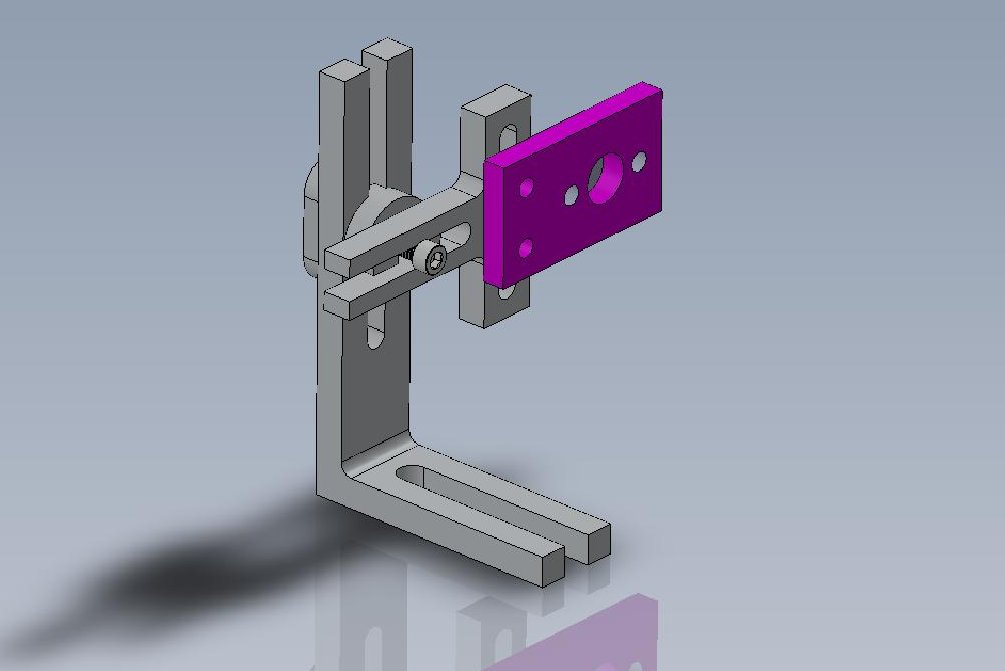
\includegraphics[width = 7.6cm]{cad1}
                \caption{}
				
        \end{subfigure}%
       ~~~~~
        \begin{subfigure}[h]{0.5\textwidth}
                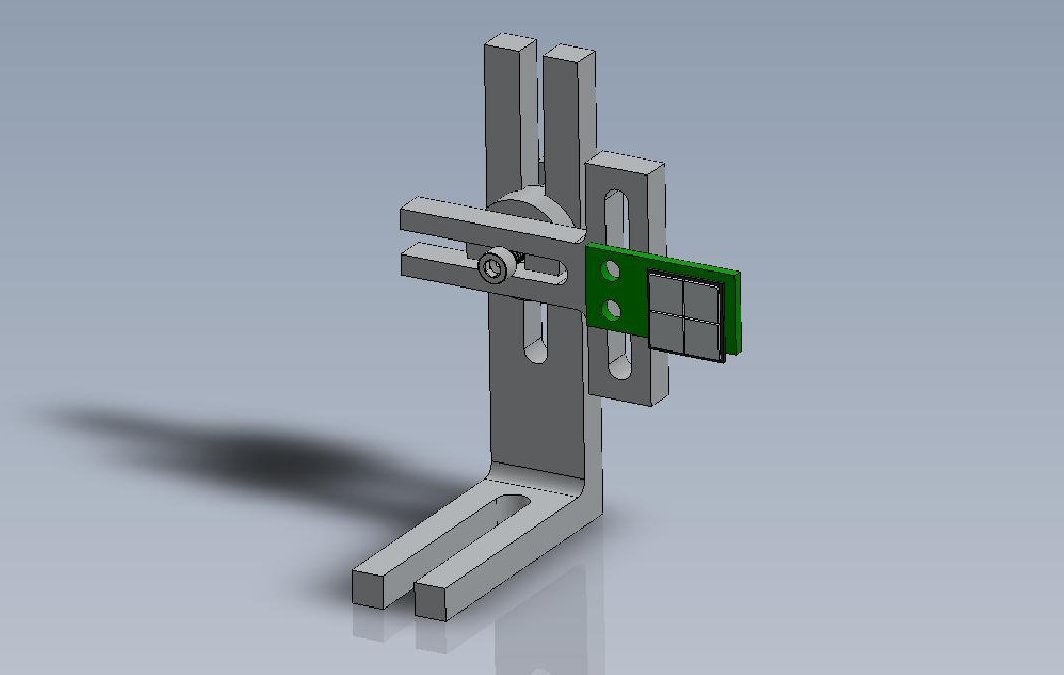
\includegraphics[width = 8cm]{cad2}
                \caption{}
                
        \end{subfigure}
        \caption{Displays the many configurations the support pieces can take on the accommodate the parameters of detector tests}
        \label{cad1}
\end{figure}


\subsection{Electronics}
There are a number of ways to read out the pixels from each array. These can be summed into two categories, Independent and multiplexing. The independent method involves reading out each pixel into its own channel. This makes for excellent resolution however, adding channel increases costs, design complexity and data output. Additionally large circuitry is required to handle even simple arrays. Multiplexing is a method used to reduce complexity and cost however can reduce timing due to the increase in capacitance  that comes with typical summing configurations. The goal is to find a healthy balance of channels, ie selecting the most one can attain given costs, timing and design constraints while minimizing the amount of multiplexing. This further shows the importance of testing the effects of multiple pixels summed together. In addition to simple summing configurations and basic biasing circuit was used for testing which originates from sensl recommended operating procedures which is displayed in figure \ref{circ}.

\begin{figure}[H]
\centering
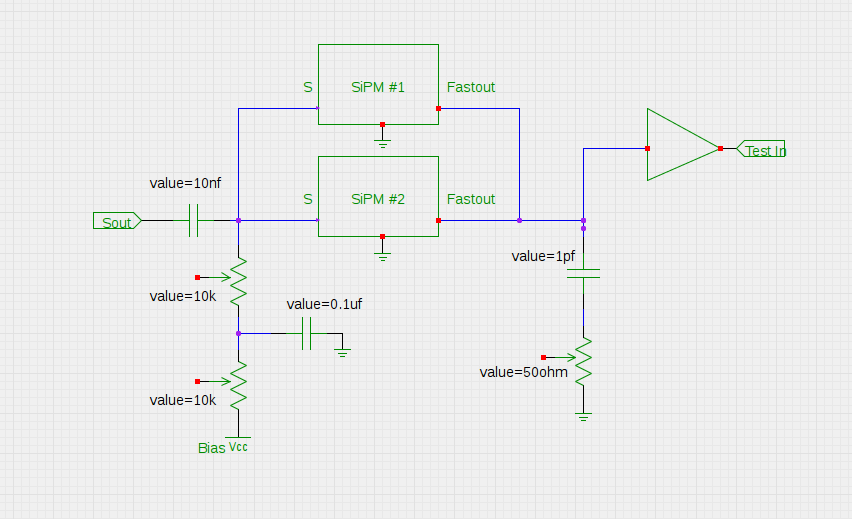
\includegraphics[width=0.80\linewidth]{circ}
\caption{Displays the biasing configuration used for C and B series devices, as well as the method for pixel multiplexing. The configuration is no different for a single pixel}
\label{circ}
\end{figure}
\subsection{Device Characterization}
Data collected during testing was analyzed using ROOT which a standard analysis program common in particle physics. All test results and ROOT macros are provided and can be found in \textit{sipmdata} folder (onedrive). Below is an outline of the tests performed for N number of pixels and $V_{ob}$ threshold levels:

1. SiPM/amplifier response function 

2. Dark counts vs. threshold

3. Time resolution (jitter) with laser (oscilloscope acquisition)

The response function of the amplified was determined by injecting a short square pulse into the 'test' input. The step response of a dynamical system gives information on the stability of such a system, and on its ability to reach one stationary state when starting from another To inject charge impulse you apply a voltage step from rectangular pulse from a pulse or function generator was a resolution of at least 80 ps. A 1 mV rectangle (step) will inject $1mV*1pF=1fC$. An SiPM pulse for the b-series is 2.6 fC per $V_{ob}=1V$.  The amplifier response is about 0.5mV/fC. 

\begin{equation}
\label{risefall2}
V(t) = V_{max} (exp(\frac{-(t-t_{o})}{\tau_{Rise}})-exp(\frac{-(t-t_{o})}{\tau_{Fall}}))
\end{equation}

Therefore a response of ~10 fC was measured which gives approximately a 5mV peak, large enough to be measured with an oscilloscope. Its important to note the bias doesn't denote the impedance of the SiPM, and the step response is only dependent on the amplitude of the step and the network time constant, which is independent of $V_{ob}$, therefore the response should also be independent of $V_{ob}$. An example of response function of the amplified taken while connected to a B-series pixel is displayed in figure \ref{resp}. The average response was fitted using root which enabled to calculation of the rise and fall times. The equation used to fit the response is displayed as equation \ref{risefall2}.

\begin{figure}[H]
\centering
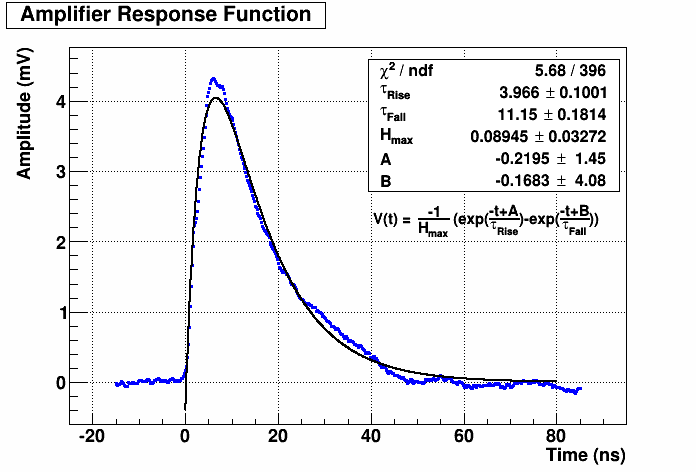
\includegraphics[width=0.70\linewidth]{resp}
\caption{Displays the biasing configuration used for C and B series devices}
\label{resp}
\end{figure}

A single photo-electric pulse was measured and fitted. This was done to characterize the rise and fall time of the SiPM which would give insight into the possible timing resolution of the spectrometer. 1000 signals were averaged and fitted which is displayed in \ref{single}

\begin{figure}[H]
        \centering
        \begin{subfigure}[h]{0.5\textwidth}
                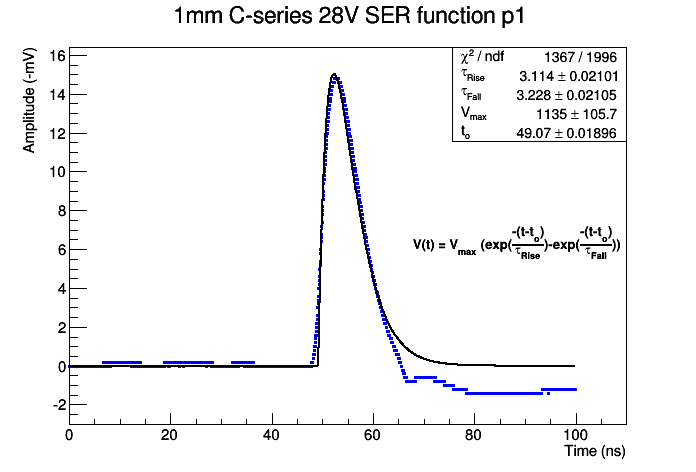
\includegraphics[width = 8cm]{fit9}
                \caption{}
				
        \end{subfigure}%
       ~
        \begin{subfigure}[h]{0.5\textwidth}
                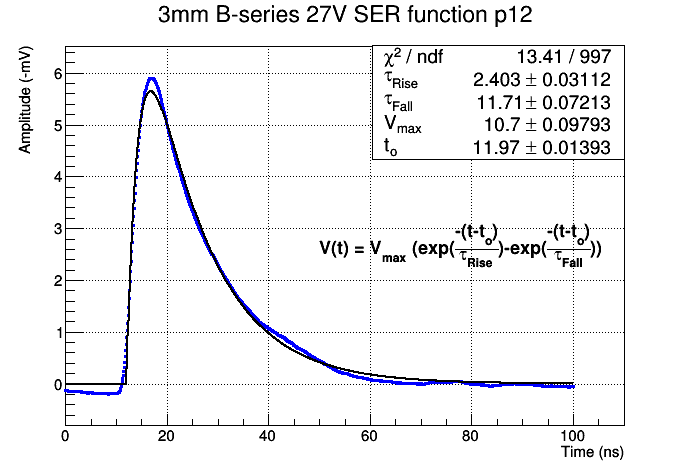
\includegraphics[width = 8cm]{fit10}
                \caption{}
                
        \end{subfigure}
        \begin{subfigure}[h]{0.5\textwidth}
                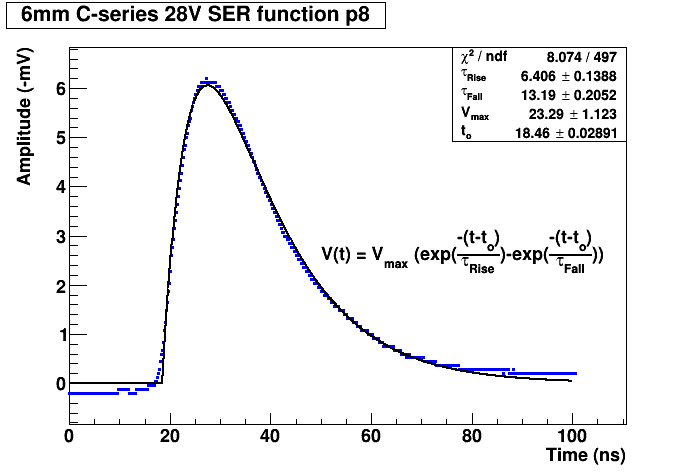
\includegraphics[width = 8cm]{fit8}
                \caption{}
                
        \end{subfigure}
        
       

        \caption{Displays the single photo-electric response of the 1mm C-series (a), the 3mm B-series (b) and the 6mm C-series (c).}
        \label{single}
\end{figure}

Additionally different number of pixels were summed together to gauge the affect of multiplexing. This is demonstrated in figure \ref{mult} which shows the single photo-electric response for 1, 2, 3, and 4 pixels. Its interesting to note the increase in rise and fall times which can be crucial in the timing performance of the spectrometer. One should notice the artifact before the pulse becomes more significant for additional pixels and ultimately discredits the fit. The fit was only found to be valid for single pixels.

\begin{figure}[h!]
        \centering
        \begin{subfigure}[h]{0.5\textwidth}
                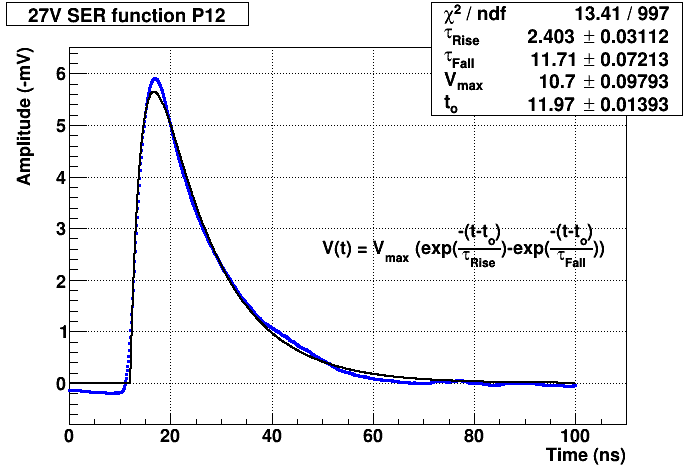
\includegraphics[width = 7cm]{fit3}
                \caption{}
				
        \end{subfigure}%
        ~     
        \begin{subfigure}[h]{0.5\textwidth}
                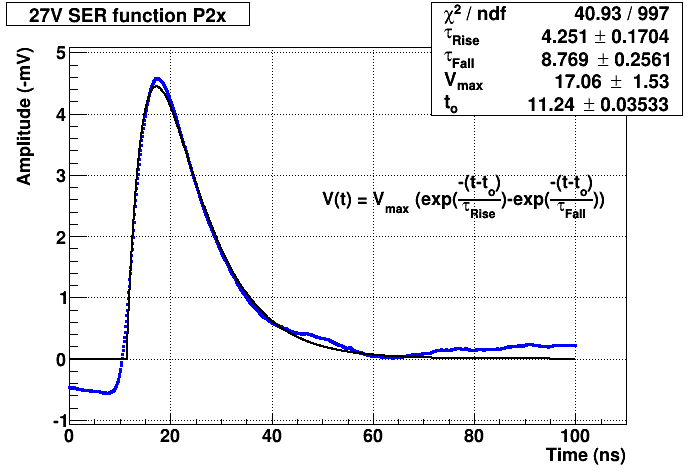
\includegraphics[width = 7cm]{px2}
                \caption{}
                
        \end{subfigure}
         
       \begin{subfigure}[h]{0.49\textwidth}
                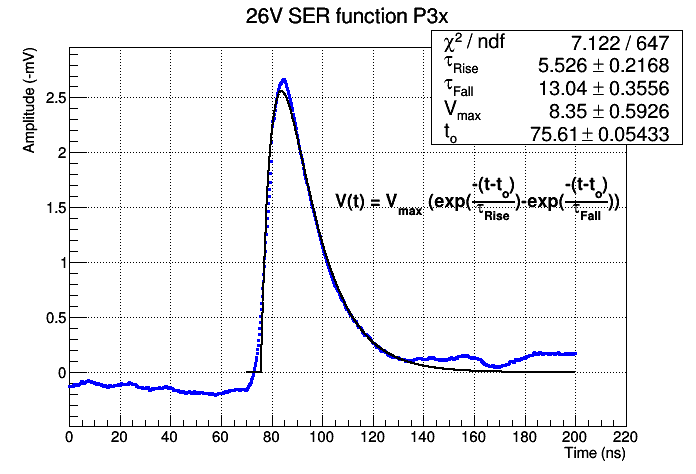
\includegraphics[width = 7cm]{px3}
                \caption{}
                
        \end{subfigure}
        ~
        \begin{subfigure}[h]{0.45\textwidth}
                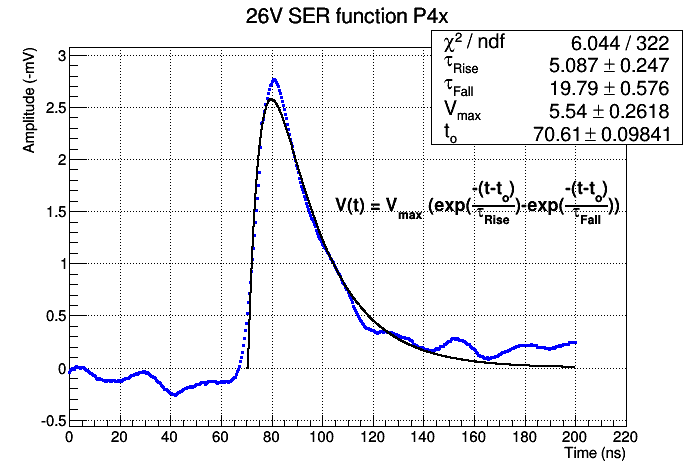
\includegraphics[width = 7cm]{px4}
                \caption{}
                
        \end{subfigure}

        \caption{Displays the effect of multiplexing on rise and fall times for B-series 3mm, (a) 1-pixel (b) 2-pixels (c) 3-pixels (d) 4-pixels. One should notice the artifact before the pulse becomes more significant for additional pixels and discredits the fit}
        \label{mult}
\end{figure}

The breakdown point of the pixel is also required to figure out the correct way to bias the detector. Breakdown was calculated by finding the relation between amplitude and $V_{ob}$ and then solving for when amplitude is zero. This is shown in figure \ref{bd}.



When detecting any signal noise to signal level is a crucial value to know. For SiPM's the noise can vary with bias and summing configuration. Using the tekvisa trace grabber, A 1000, 400ns traces were captured and analyzed for pulse frequency for 1,2,3 and 4 PE thresholds as well as for pixel multiplexing. Two different pulse detection methods were used; The first based solely on threshold, and the other based on pulse amplitude, displayed in figure \ref{dn}.

The "trigger" charts show all signals with a specific amplitude at a particular threshold which exclude hits above an "upper limit", while the "threshold" will show all hits that occur at and above a specific threshold. This data can not only be used for determination of noise frequencies at different thresholds it can be used to help determine the range of particular amplitudes for different photo-electron levels.


The results of the noise tests on the final devices will help determine the ideal biasing levels and amplification. Additional tests included investigation of the intrinsic resolution of the SiPM's. The can be found by firing a short laser pulse ~80ps into the device and looking at the consistency of the timing from the output signal. The spread of the timings ultimately determine the intrinsic timing of SiPM and amplifier which will exclude timing affects due to geometry and positron energy. This was measured using oscilloscope acquisition for the B-series only (C-series was measured using VME) which is display in figure \ref{l1} and \ref{l2}. 

The results found indicate that high resolution can be attained for the B-series given the energy of the positron is high enough (>100pe per array) to provide a high intensity light burst and given an optimal bias threshold (~27V) is used.

\newpage
\begin{figure}[H]
        \centering
        \begin{subfigure}[h]{0.5\textwidth}
                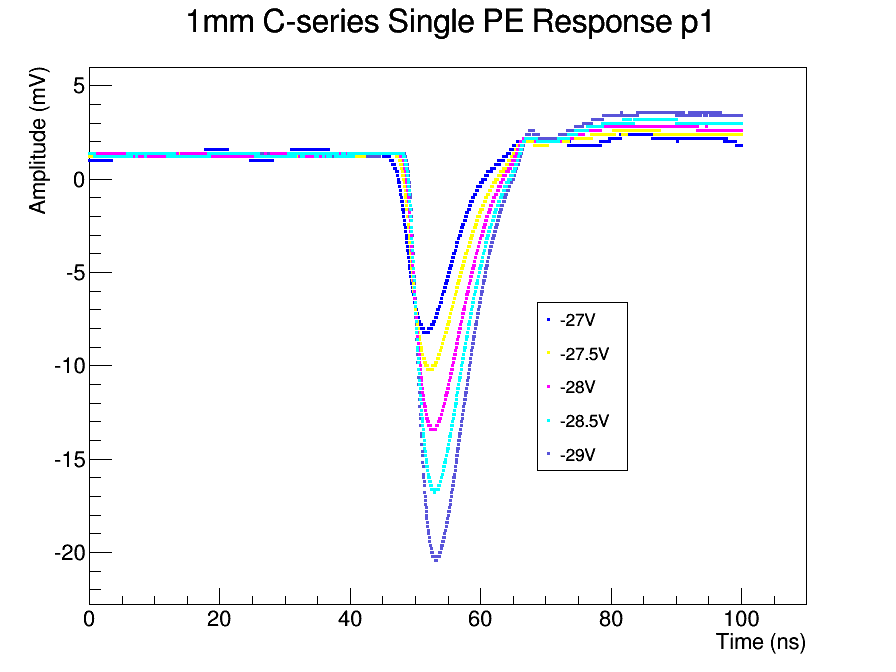
\includegraphics[width = 8cm]{bd5}
                \caption{}
				
        \end{subfigure}%
       ~
        \begin{subfigure}[h]{0.5\textwidth}
                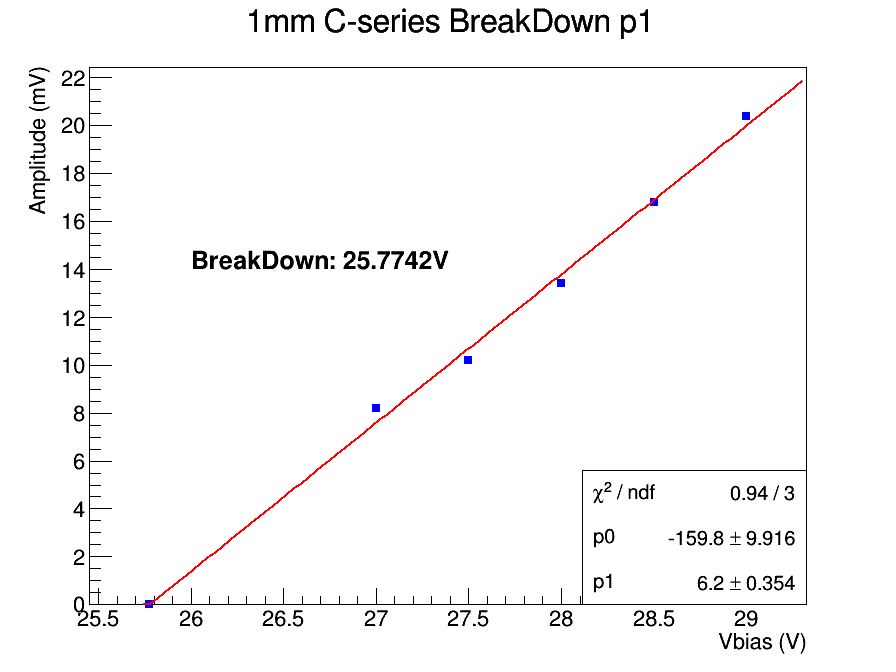
\includegraphics[width = 8cm]{bd6}
                \caption{}
                
        \end{subfigure}
                \begin{subfigure}[h]{0.5\textwidth}
                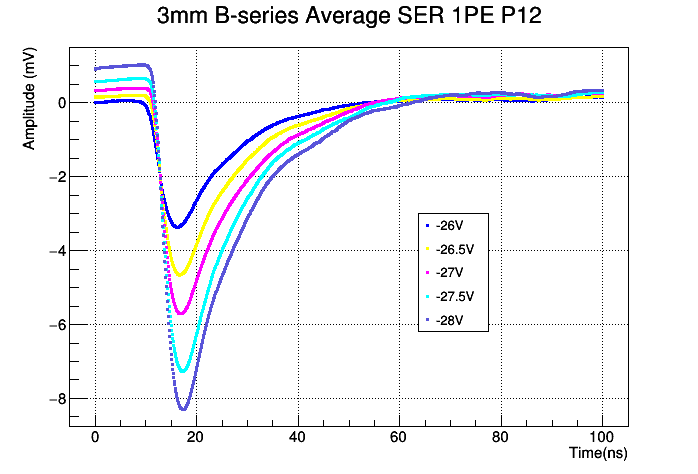
\includegraphics[width = 8cm]{bd1}
                \caption{}
				
        \end{subfigure}%
       ~
        \begin{subfigure}[h]{0.5\textwidth}
                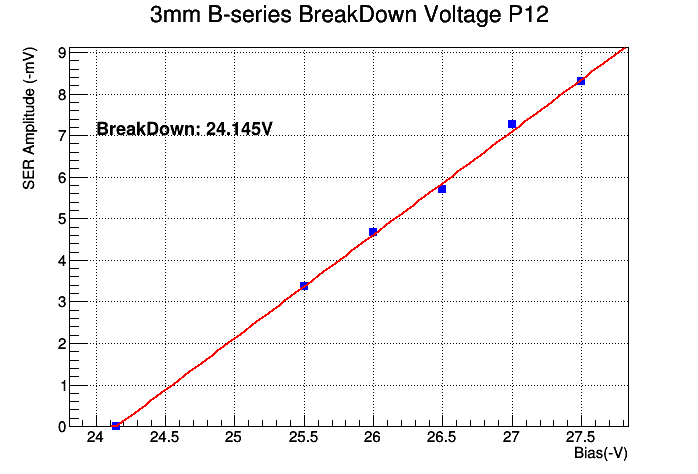
\includegraphics[width = 8cm]{bd2}
                \caption{}
                
        \end{subfigure}
                \begin{subfigure}[h]{0.5\textwidth}
                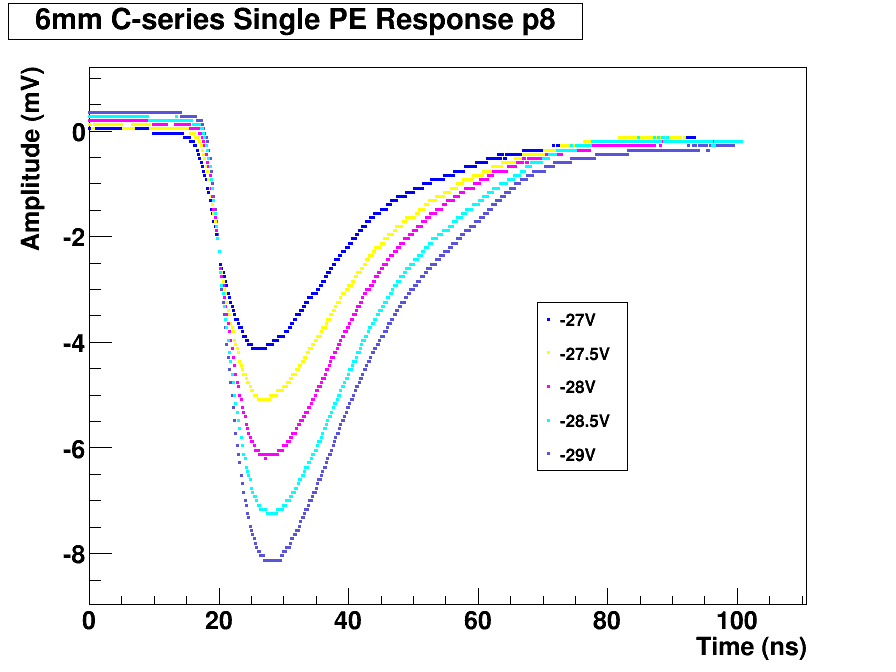
\includegraphics[width = 8cm]{bd3}
                \caption{}
				
        \end{subfigure}%
       ~
        \begin{subfigure}[h]{0.5\textwidth}
                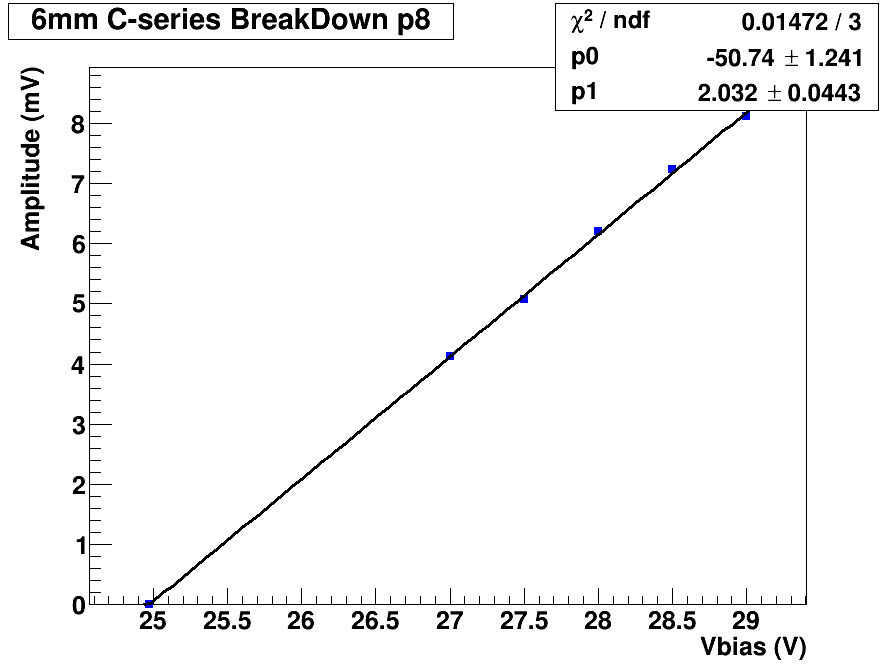
\includegraphics[width = 8cm]{bd4}
                \caption{}
                
        \end{subfigure}
        
       

        \caption{The (a),(c) and (e) figures display the signals collected and used to calculate the breakdown voltage of figures (b),(d) and (f) for 1mm, 3mm and 6mm devices respectively}
        \label{bd}
\end{figure}

\begin{figure}[H]
        \centering
        \begin{subfigure}[h]{0.45\textwidth}
                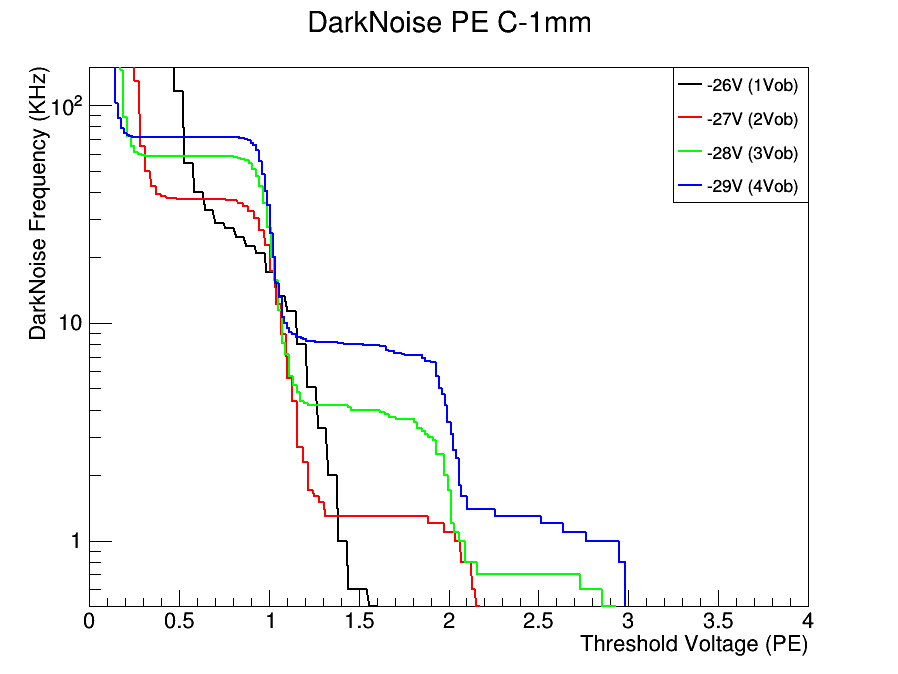
\includegraphics[width = 7cm]{dn4}
                \caption{}
				
        \end{subfigure}%
        \begin{subfigure}[h]{0.45\textwidth}
                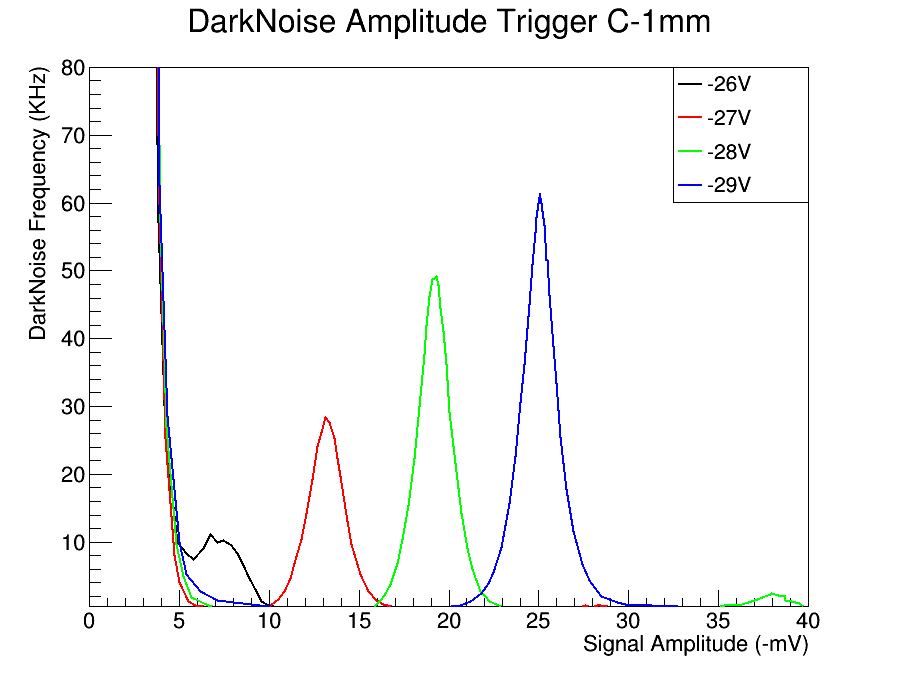
\includegraphics[width = 7cm]{dn6}
                \caption{}
                
        \end{subfigure}               
        \begin{subfigure}[h]{0.45\textwidth}
                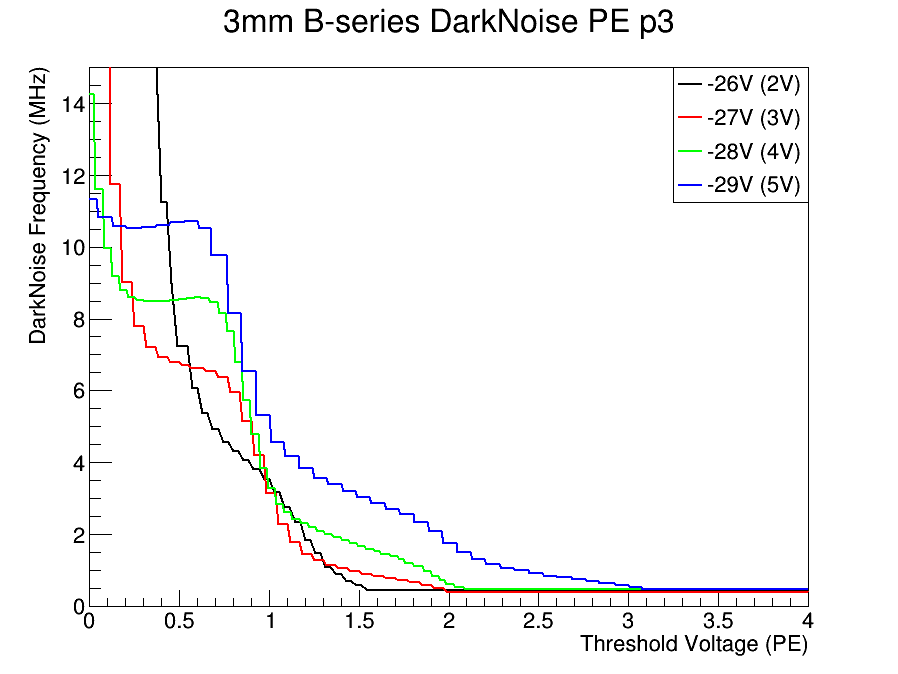
\includegraphics[width = 7cm]{dn1}
                \caption{}
          \end{subfigure}               
         \begin{subfigure}[h]{0.45\textwidth}
                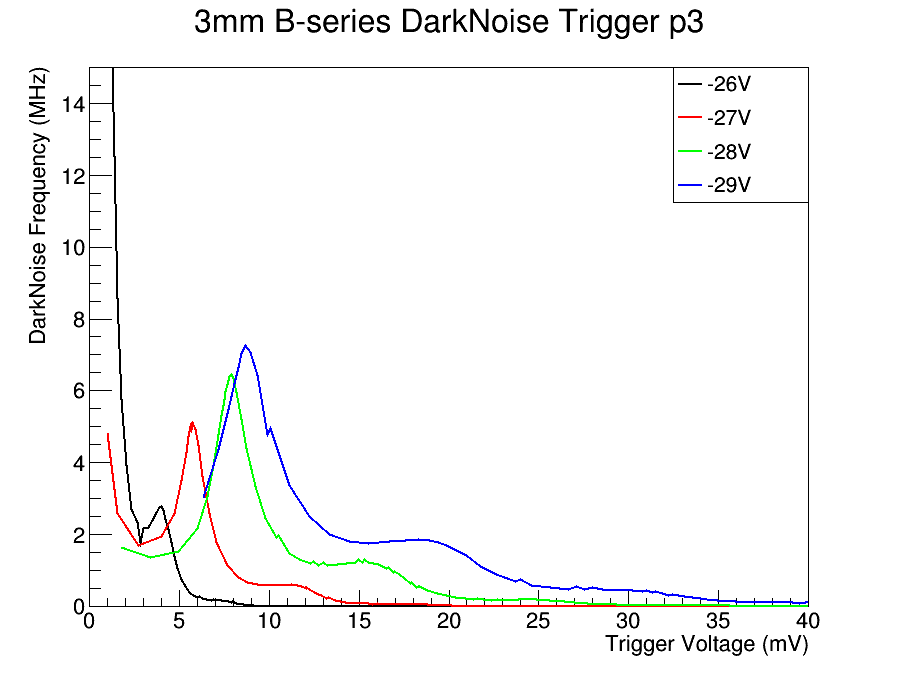
\includegraphics[width = 7cm]{dn3}
                \caption{}
           \end{subfigure}    
           \begin{subfigure}[h]{0.45\textwidth}
                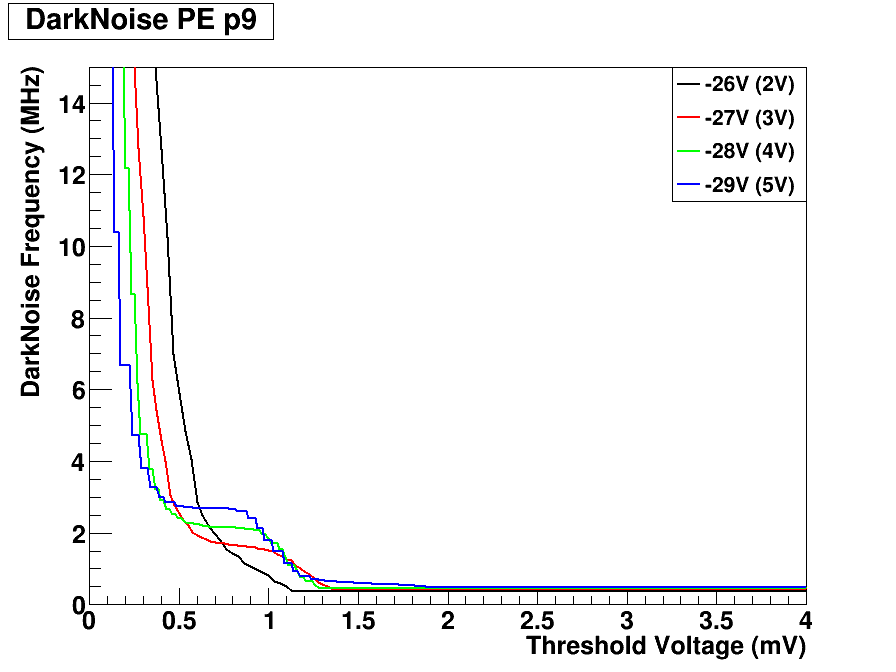
\includegraphics[width = 7cm]{dn7}
                \caption{}
          \end{subfigure}               
         \begin{subfigure}[h]{0.45\textwidth}
                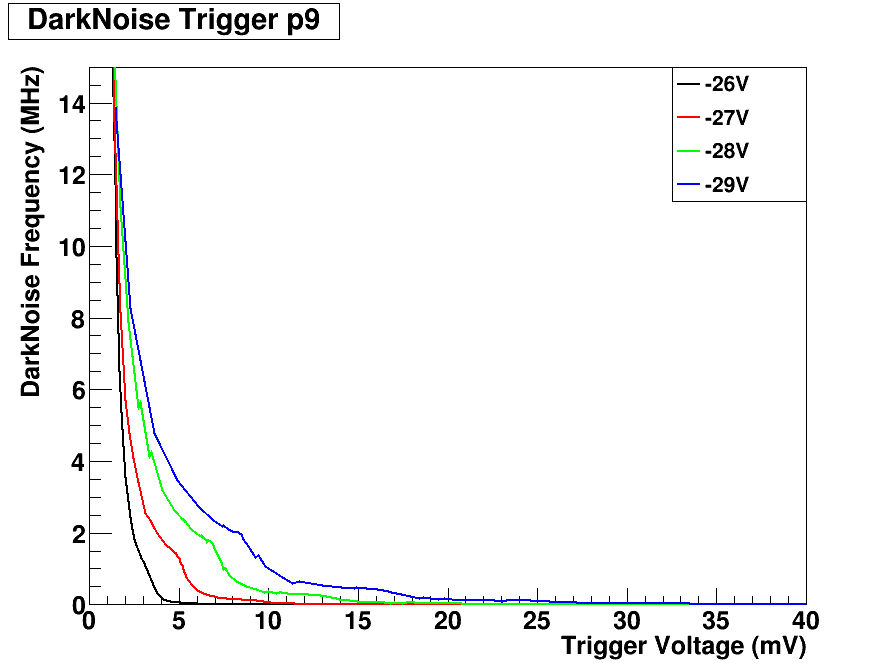
\includegraphics[width = 7cm]{dn9}
                \caption{}
              
        \end{subfigure}

        \caption{Displays the darknoise data collected from a 1mm, 3mm and 6mm pixels. Figures a) c) and e) displays threshold noise normalized in photo-electrons while figures b) d) and f) Shows noise triggers with a specific amplitude for 1mm, 3mm and 6mm pixels respectively. It should be noted that the 1mm is in kHz while the 3mm and 6mm are in MHz}
        \label{dn}
\end{figure}

\begin{figure}[H]
        \centering
        \begin{subfigure}[h]{0.5\textwidth}
                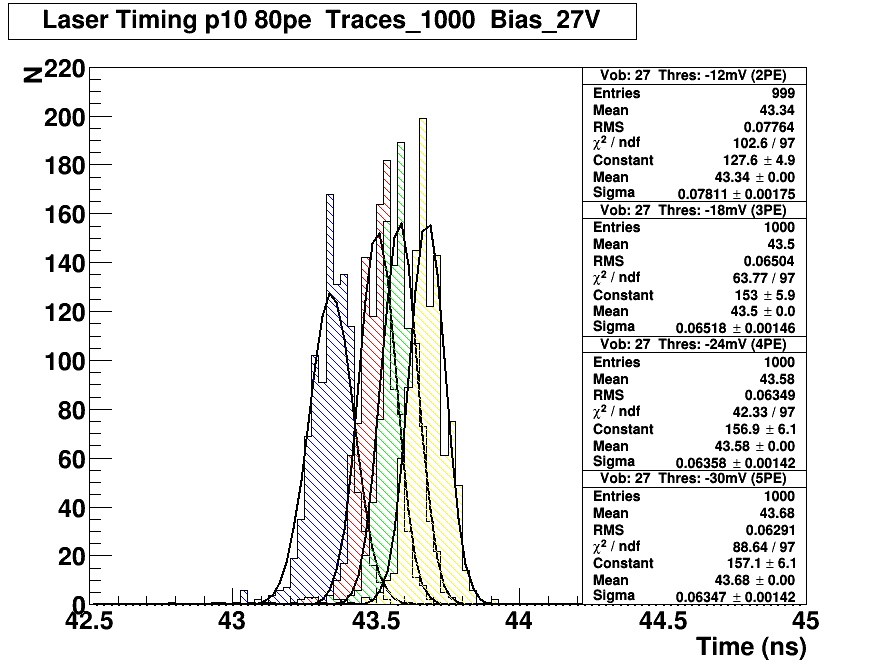
\includegraphics[width = 7cm]{l80}
                \caption{}
				
        \end{subfigure}% 
        ~~     
        \begin{subfigure}[h]{0.5\textwidth}
                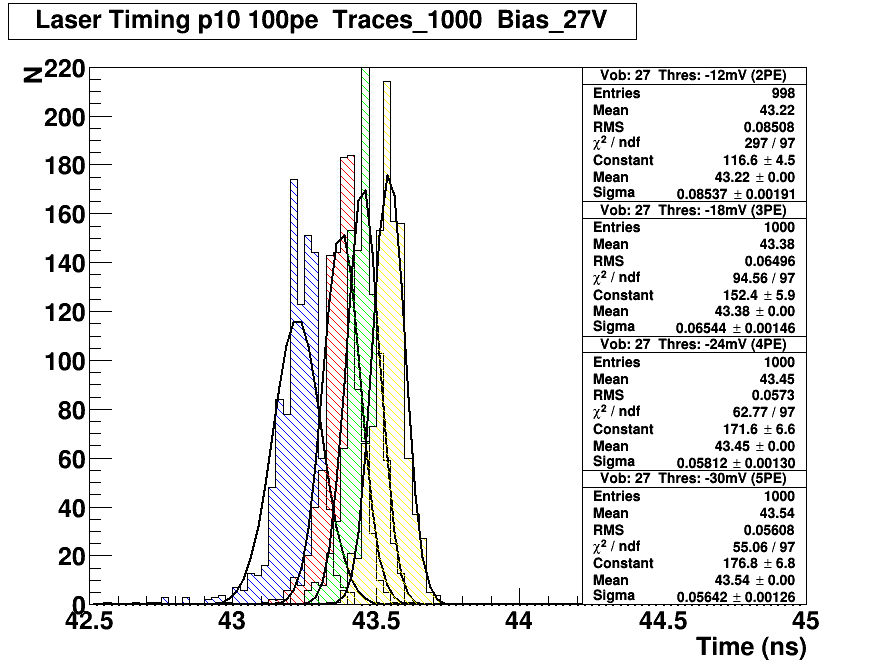
\includegraphics[width = 7cm]{l100}
                \caption{}
                
        \end{subfigure}       
       \begin{subfigure}[h]{0.5\textwidth}
                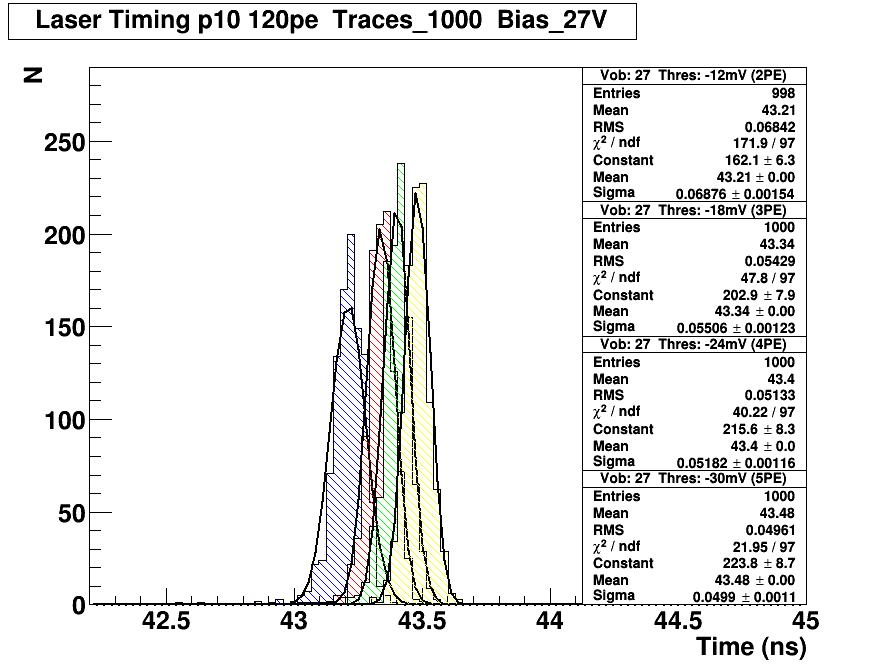
\includegraphics[width = 7cm]{l120}
                \caption{}
                
        \end{subfigure}
  

        \caption{Displays the effect of applying different laser intensity levels (80pe, 100pe, 120pe) has on the timing of the detected signal for 3mm B-series (non-TDC)}
        \label{l1}
\end{figure} 

\begin{figure}[H]
        \centering
        \begin{subfigure}[h]{0.5\textwidth}
                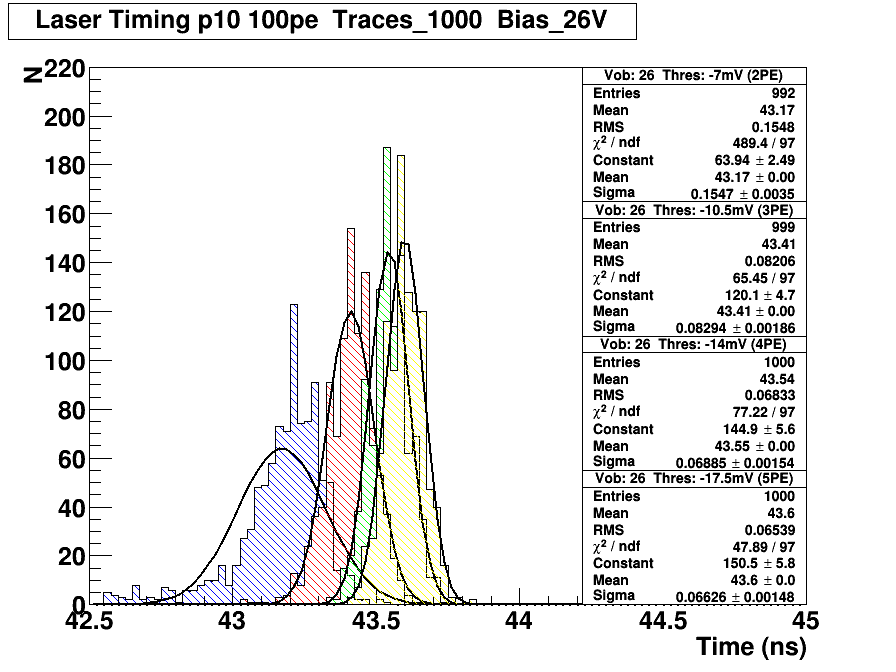
\includegraphics[width = 7cm]{laz1}
                \caption{}
				
        \end{subfigure}%
       ~~
        \begin{subfigure}[h]{0.5\textwidth}
                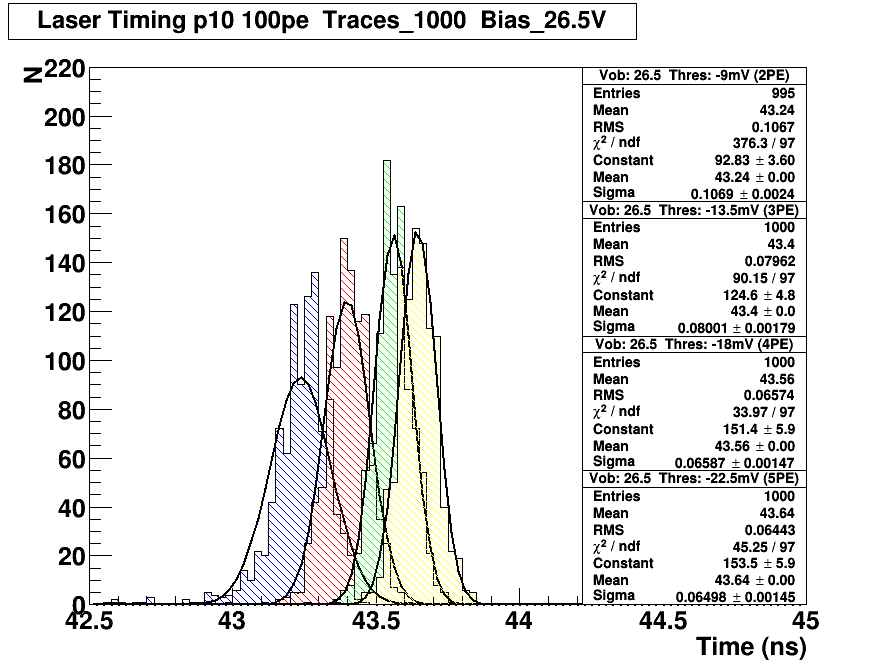
\includegraphics[width = 7cm]{laz2}
                \caption{}
                
        \end{subfigure}
        
       \begin{subfigure}[h]{0.5\textwidth}
                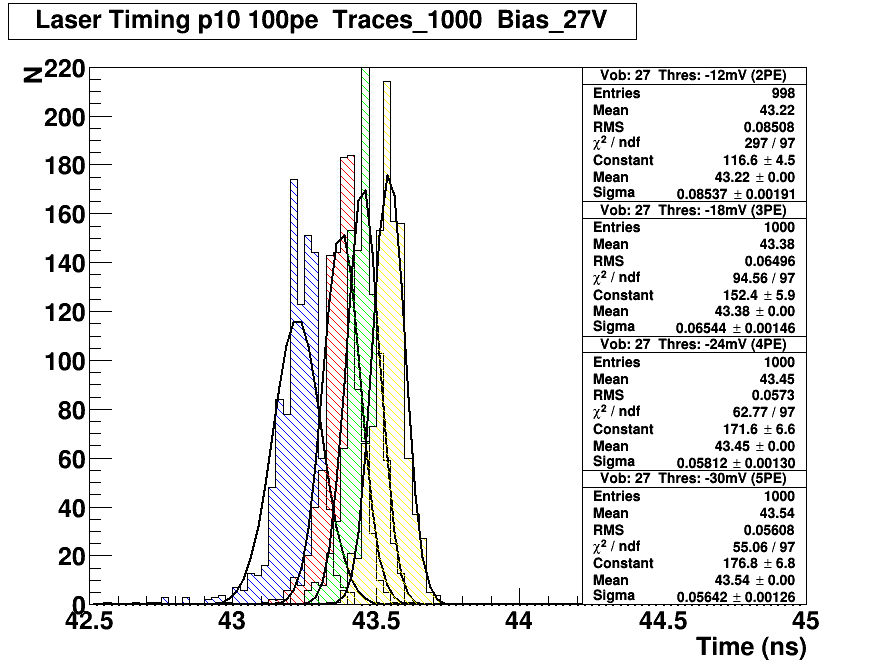
\includegraphics[width = 7cm]{laz3}
                \caption{}
                
        \end{subfigure}
  

        \caption{Displays the effect of applying different bias thresholds (26V, 26.5V, 27V) on the timing of the detected signal for 3mm B-series (non-TDC)}
        \label{l2}
\end{figure} 
\newpage

\subsection{Timing Resolution VME}
A large part of my time in M9 project was spent trying to determine and/or improve the timing resolution of the final spectrometer. Ultimately the project came down to a competition between two methods of collecting signals. The first and formally the regular way of acquiring timing is the constant fraction method. This method sums signals from pixel arrays together using fan in/outs, then uses a constant fraction discriminator to generate a timing pulse to be read by the TDC. In the second method, formally known as \textit{Leonids method} timing signals are generated by triggers via a 3rd or 4rth photo-electron using a threshold discriminator built into the pre-amp. Signals are fed directly into an OR and an AND gate. The OR signal is fed into the TDC and together with charge and amplitude information from the QDC the time is corrected using software, while the AND gate is used for coincidence.

\begin{figure}[H]
\centering
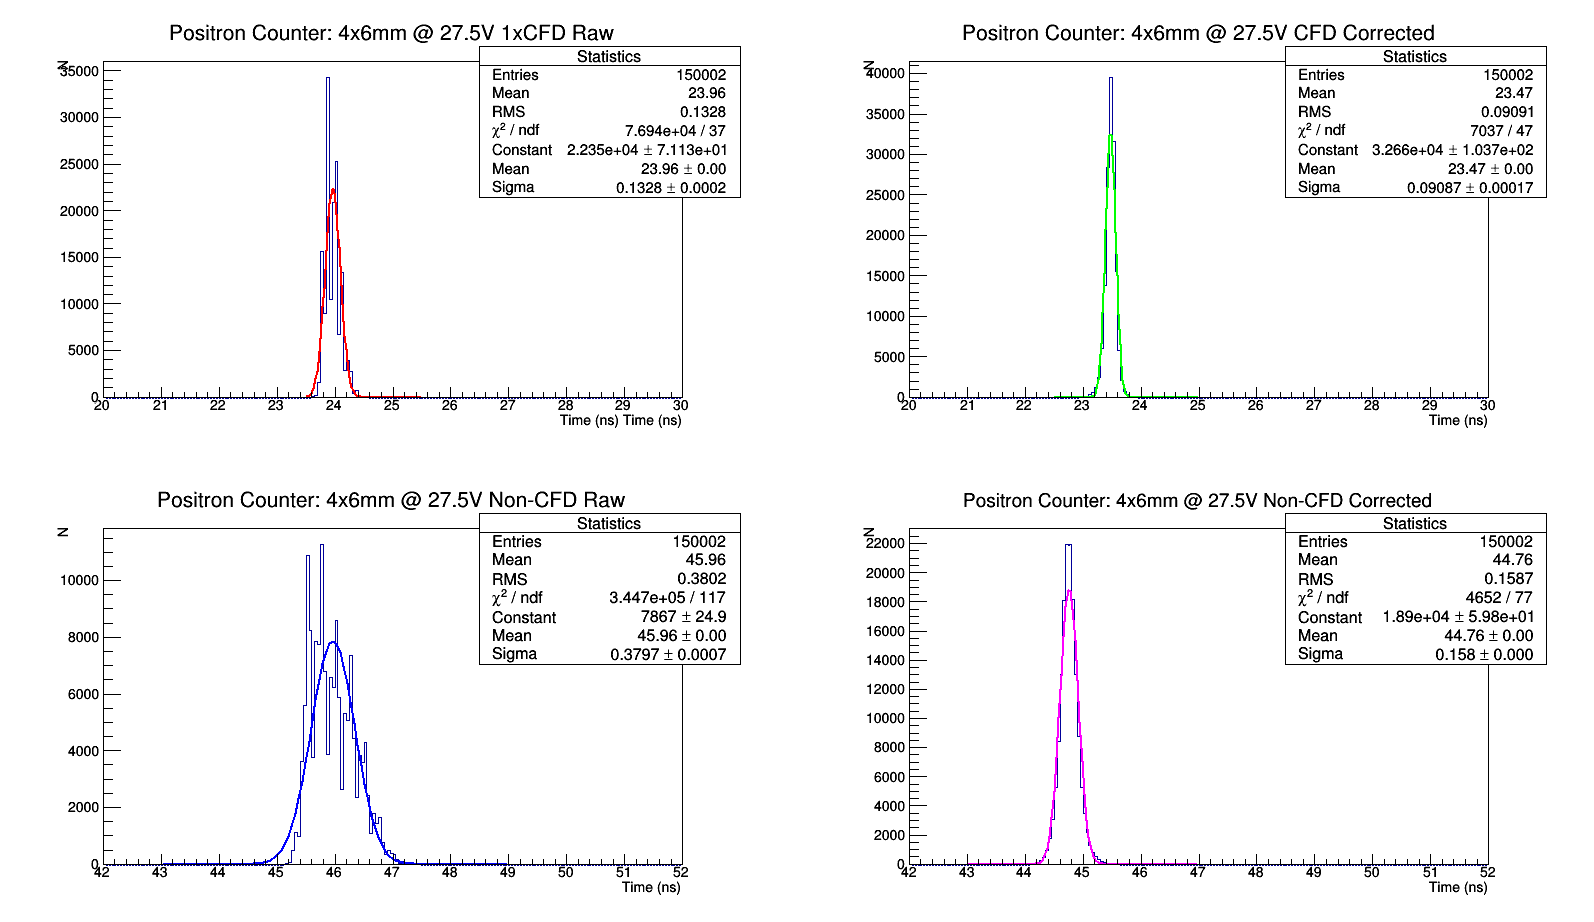
\includegraphics[width=1.10\linewidth]{comp1}
\caption{Displays the Timing resolution comparison between Leonids Method (non-CFD) and CFD method. Both in this case had an amplitude dependence that was correct using software}
\label{comp}
\end{figure}

 The two methods were tested extensively through-out the duration of this project, with each method being refined for optimum resolution. To test the resolution of each method a laser pulse is generated and fed into a 4x6mm pixel array via a rectangular light guide. This ensures all the light reaches the array for each run. The laser generates start pulse which is used as a trigger for the electronics as well as the main reference for the TDC (ch 0). The signals from the laser pulses are collected and timed used methods 1 and 2, allowing for a timing comparison. Its should be noted that Leonids method uses a curve correction. The parameters for this curve are measurement prior to data acquisition, without changing the experimental setup. ie conditions don't change. Typical comparison begins with measuring the raw data. This is then used to generate a fitted curve for which parameters are extracted. A new data run is then started with these parameter correcting the incoming time stamps. A comparison between Leonids method and Constant fraction method is display in figure \ref{comp}. The sigma value is essentially the measure of timing resolution for this measurement. The Constant Fraction Method for this setup was found to obtain the highest resolution.
\subsection{Curve Correction}
Early in the characterization process it was notice and predicted that the time stamp of the incoming signal may have a amplitude dependence. To improve the resolution a simple correction scheme was devised. By plotting the time stamp and integrated charge of a particular run in a 2D histogram a dependence could be characterized.


\begin{figure}[H]
\centering
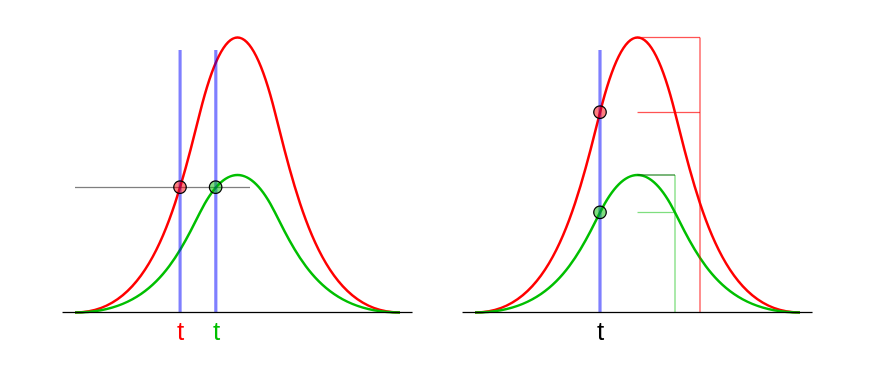
\includegraphics[width=1.10\linewidth]{const}
\caption{Displays the concept of "time walk" induced by threshold discrimination. Constant Fraction Discrimination trigger times are independent from peak heights}
\label{const}
\end{figure}

 It was known that Leonids method would require a correction. The relatively slow rise times of the signals compared to the resolution of the TDC causes a dependence of the trigger time on the signal's peak height, an effect called time walk, shown in figure \ref{const}. Constant Fraction Discrimination should overcome this deficit by essentially normalizing all the signal heights by cutting and amplifying parts of the signal. Identical rise times and peak shapes are triggered not on a fixed threshold but on a constant fraction of the total peak height, yielding trigger times independent from peak heights. It is by this method the time stamps in theory are amplitude/charge independent. However experimental data has shown that even the CFD suffers from a small amplitude or integrated charge dependence. Figure \ref{curve} displays the dependence found between time and integrated charge for both Leonids method and Constant Fraction method. 
 
\begin{figure}[H]
        \centering
        \begin{subfigure}[h]{0.5\textwidth}
                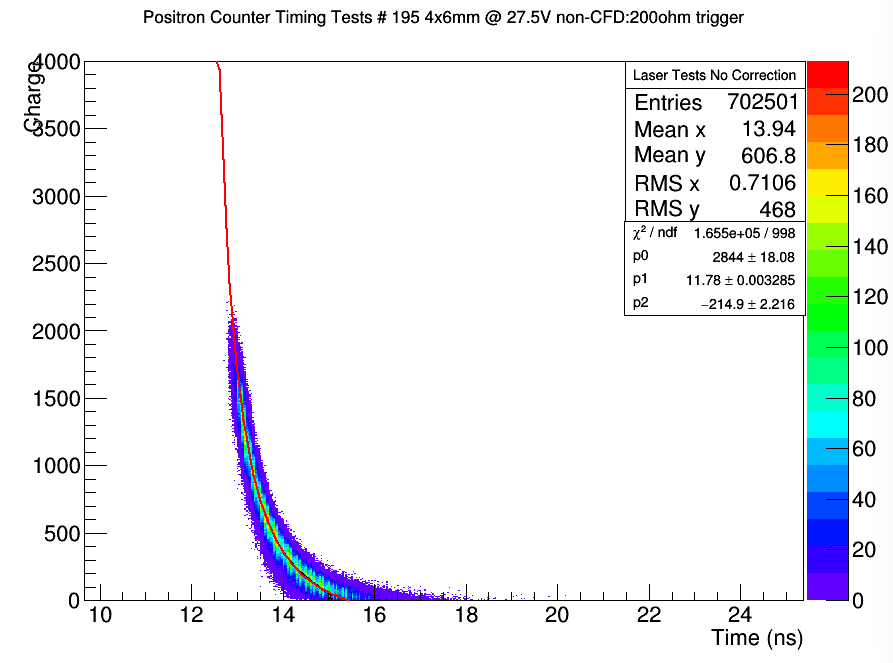
\includegraphics[width = 7cm]{cur2}
                \caption{}
				
        \end{subfigure}%
       ~~~~~
        \begin{subfigure}[h]{0.5\textwidth}
                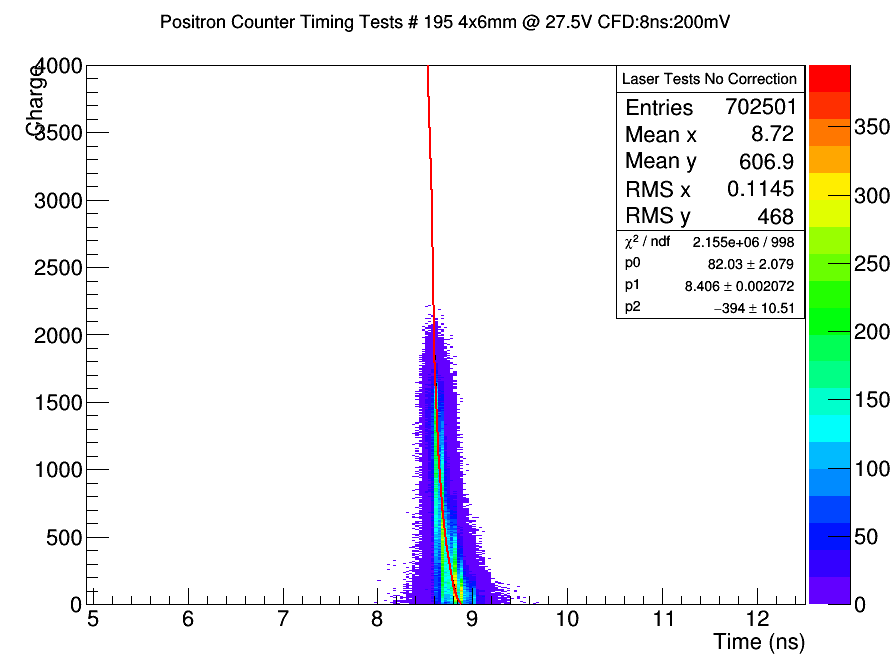
\includegraphics[width = 7cm]{cur1}
                \caption{}
                
        \end{subfigure}
        
       

        \caption{Displays the dependence found between time and integrated charge for both Leonids Method (a) and Constant Fraction method (b). The fit parameters p0 and p2 were used for corrections}
        \label{curve}
\end{figure} 

It was found that the curve commonly had a $\frac{1}{t^2}$ dependence. The full equation used for the fit is display as equation \ref{ts}.

\begin{equation}
\label{ts}
V(t)= \frac{p_0}{(t-p_1)^2}+p_2
\end{equation}

Once the parameters were calculated the times were adjusted in the midas analyzer using equation \ref{ts2} where $V$ is the measured charge from the QDC, $t$ is the uncorrected TDC measurement and $t_c$ is the corrected time.

\begin{equation}
\label{ts2}
t_c= t-\Bigg(\frac{\sqrt{p_0}}{\sqrt{V-p_2}}+p1\Bigg)
\end{equation}

This equation can be seen being implemented via the following lines of code in the \textit{T2DHistogram.cxx} script. The ROOT scripts used for fitting the 2D histograms are located in the \textit{/sipmdata/counter} directory or on the onedrive.
\begin{lstlisting}
if(TDCfdata.size() == 2 && QDCfdata.size() == 2)
{	
    for(unsigned int i = 0; i < 2; i++)
	{
	    float data1 = QDCfinaldata.at(i);	
	    float data2 = (TDCfinaldata.at(i)-tRef2) * 0.025;

		fcount = GetHistogram(i)->GetEntries();
		if(atten <= 26 && fcount <= fcount2)	
		  {float pp0, pp1, pp2;
		  GetHistogram(i)->Fill((data2), (data1));
		  //curve correction 
		    float dataC;
			float pp0 = 10900, pp1 = 0, pp2 = -5138;//curve correction pars
			dataC = data2 -((sqrt(pp0)/sqrt(data1-pp2))+pp1);
			GetHistogram(i+2)->Fill((dataC), (data1));
		  }	      
	}
}	
\end{lstlisting}
As demonstrated by the data collected in figure \ref{comp} corrections of time stamps for both Leonids Method and CFD method yield moderate to major timing improvements. However the root of the dependence seen in the CFD is not yet well understood.

\begin{figure}[H]
\centering
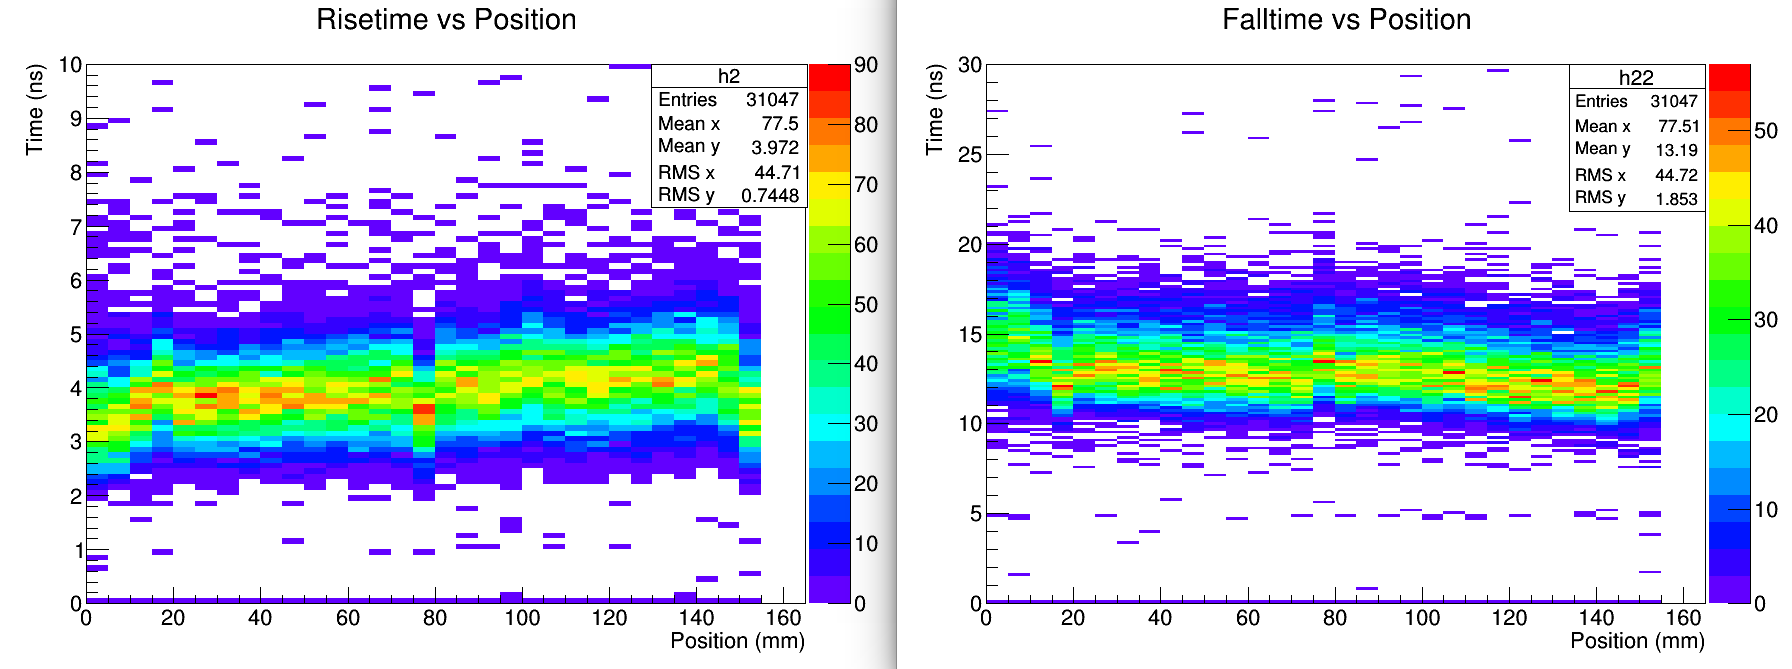
\includegraphics[width=1.10\linewidth]{ri}
\caption{Displays temporal dependence on signal rise and fall times. X-axis is distance or particle scintillation from sipm detector}
\label{ri}
\end{figure}

 The standing theory is it derives from the signal shape inconsistencies perhaps induced by a non-linear relation between signal rise time and amplitude, a measurement that has yet to be conducted. Also another artifact that may need to be taken into account when considering the best timing scheme is temporal dependence on signal shape. This is illustrated in figure \ref{ri} with the varying rise and fall time of the signal relative to positron/muon trajectory through scintillator. 


\section{Spectrometer Tests}
During the final stages of the term a mini spectrometer was designed to test the validity of our proposed best setup. This spectrometer consistence of a fully assembled muon counter and 1/8th of the planned positron counter. In order to properly collimate the beam and to help reduce backgrounds, beryllium pucks were place in strategic locations. Most of the spectrometer was designed to be 3D printed therefore designs should only be used at the most for future reference of machined parts.Figure \ref{spect} displays the cutaway renderings.

\begin{figure}[H]
        \centering
        \begin{subfigure}[h]{0.5\textwidth}
                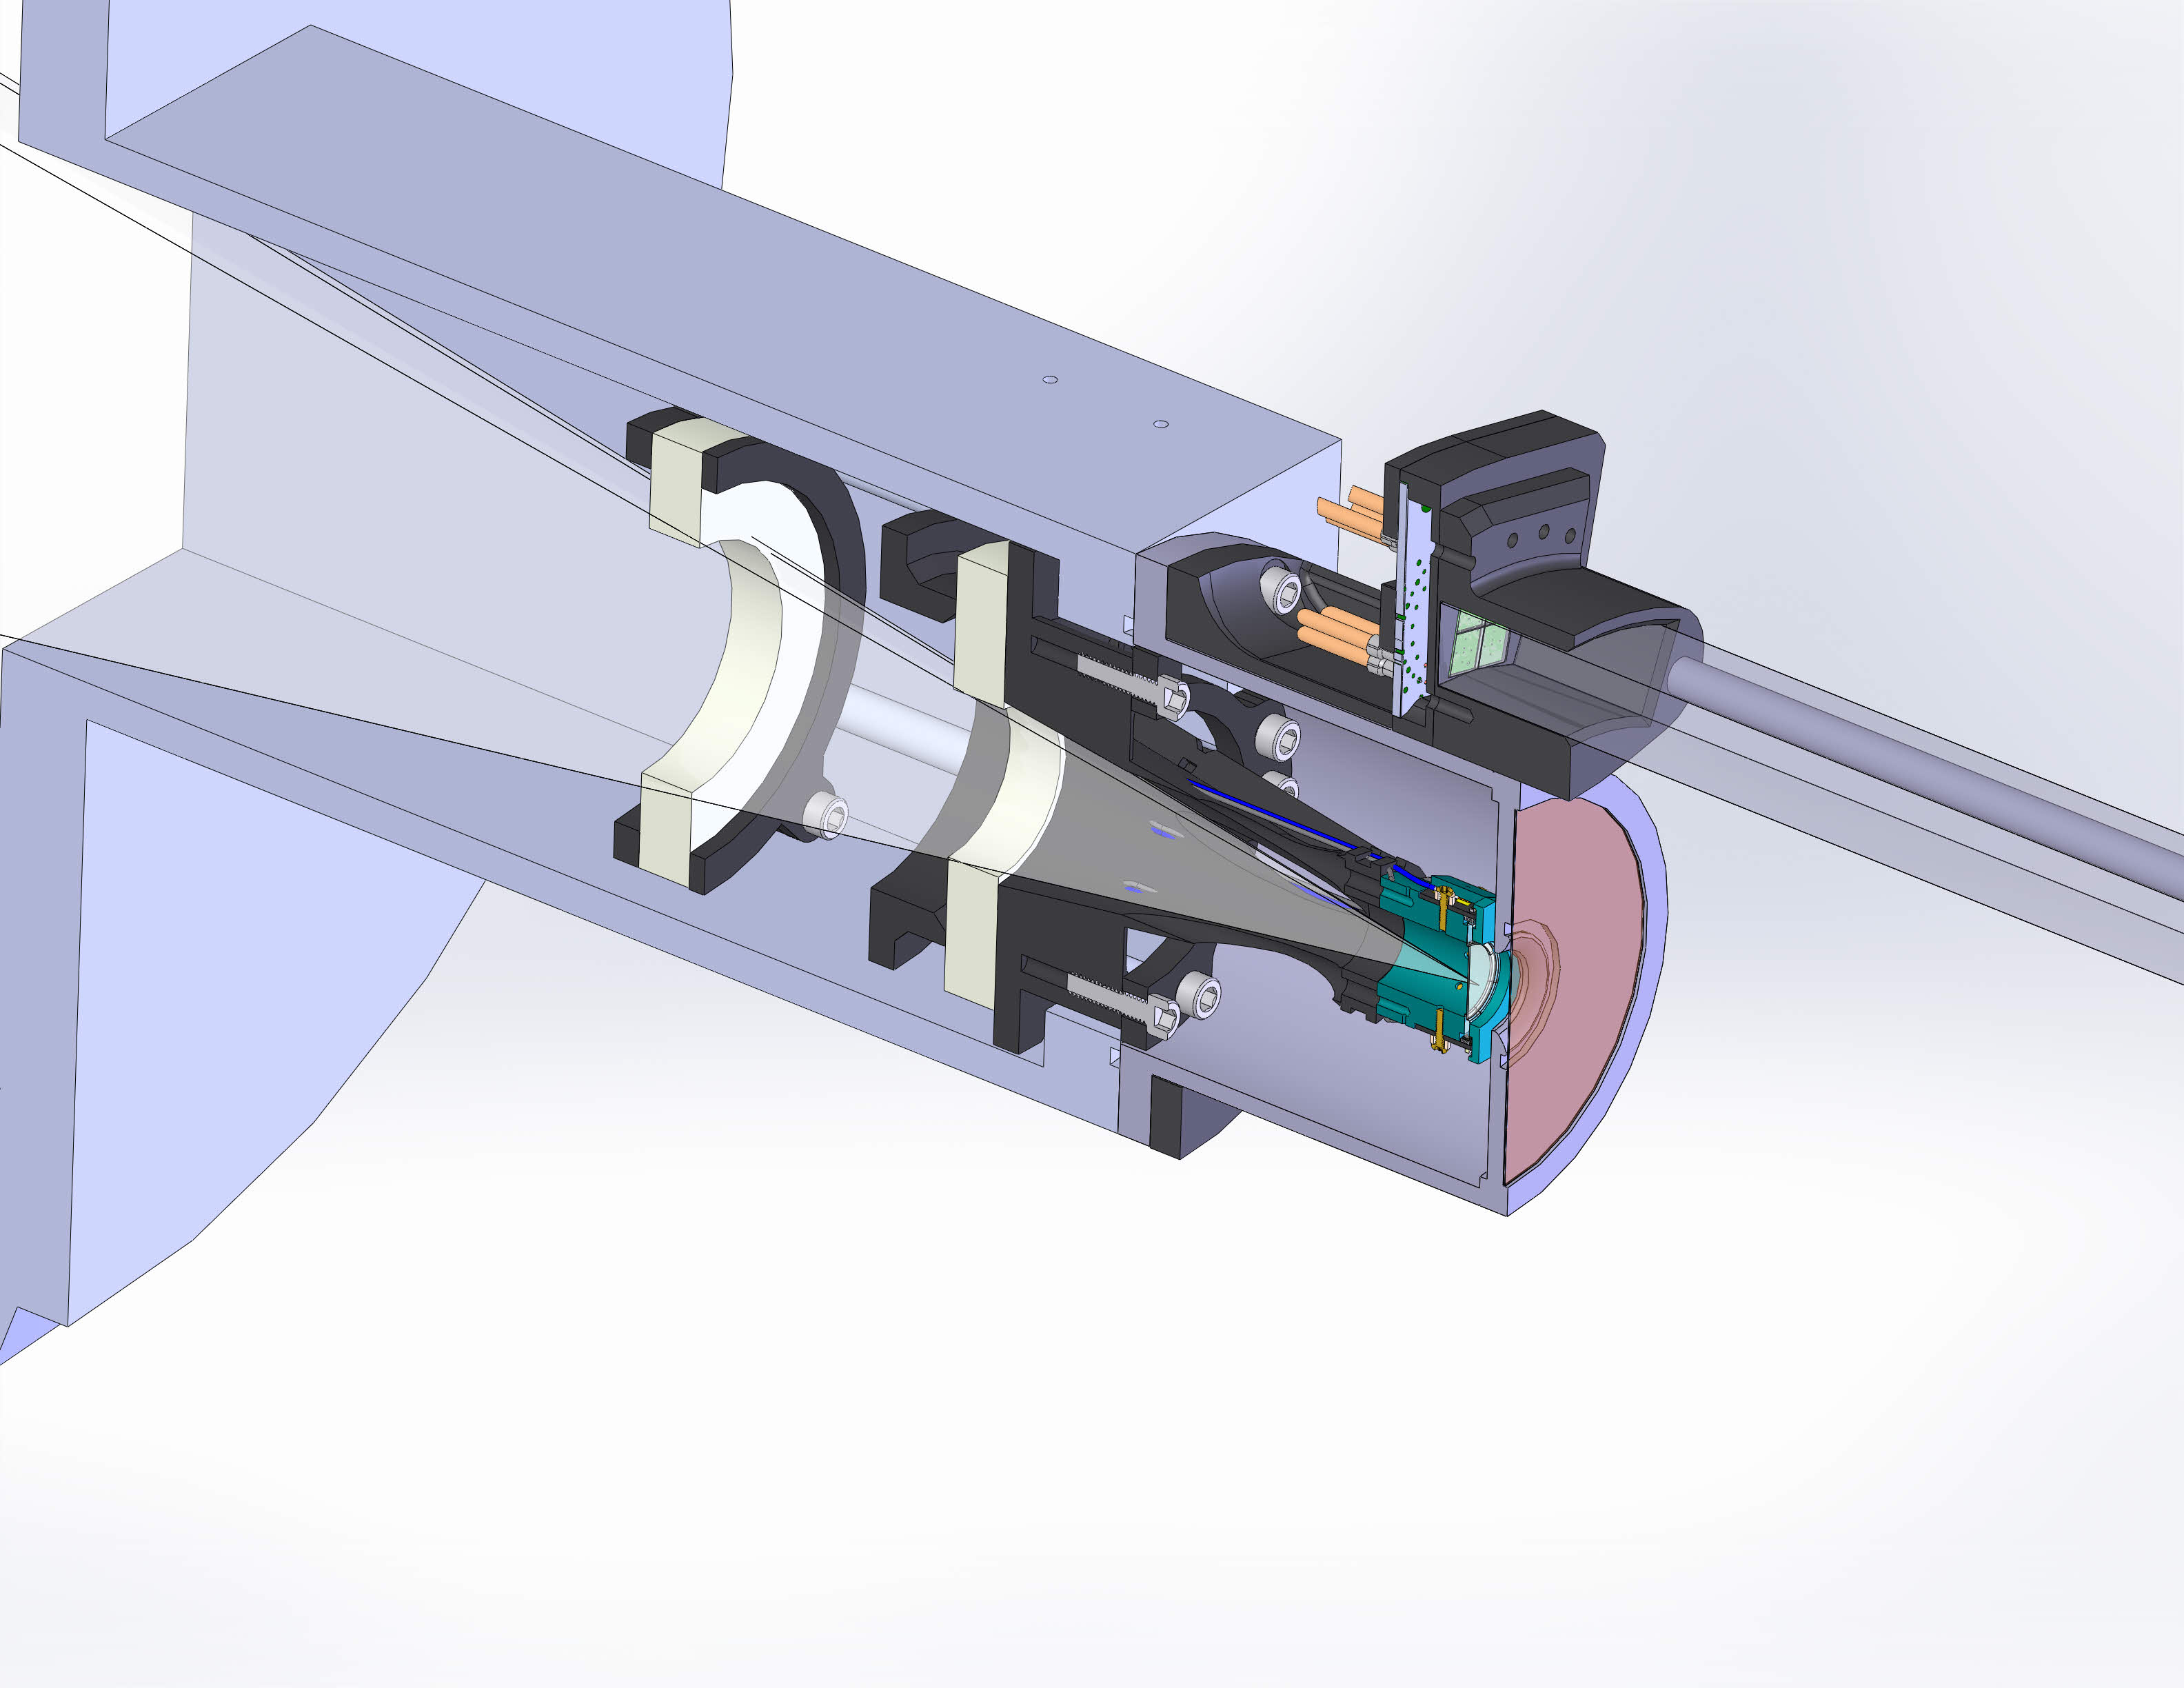
\includegraphics[width = 7cm]{sl}
                \caption{}
				
        \end{subfigure}%
       ~~~~~
        \begin{subfigure}[h]{0.5\textwidth}
                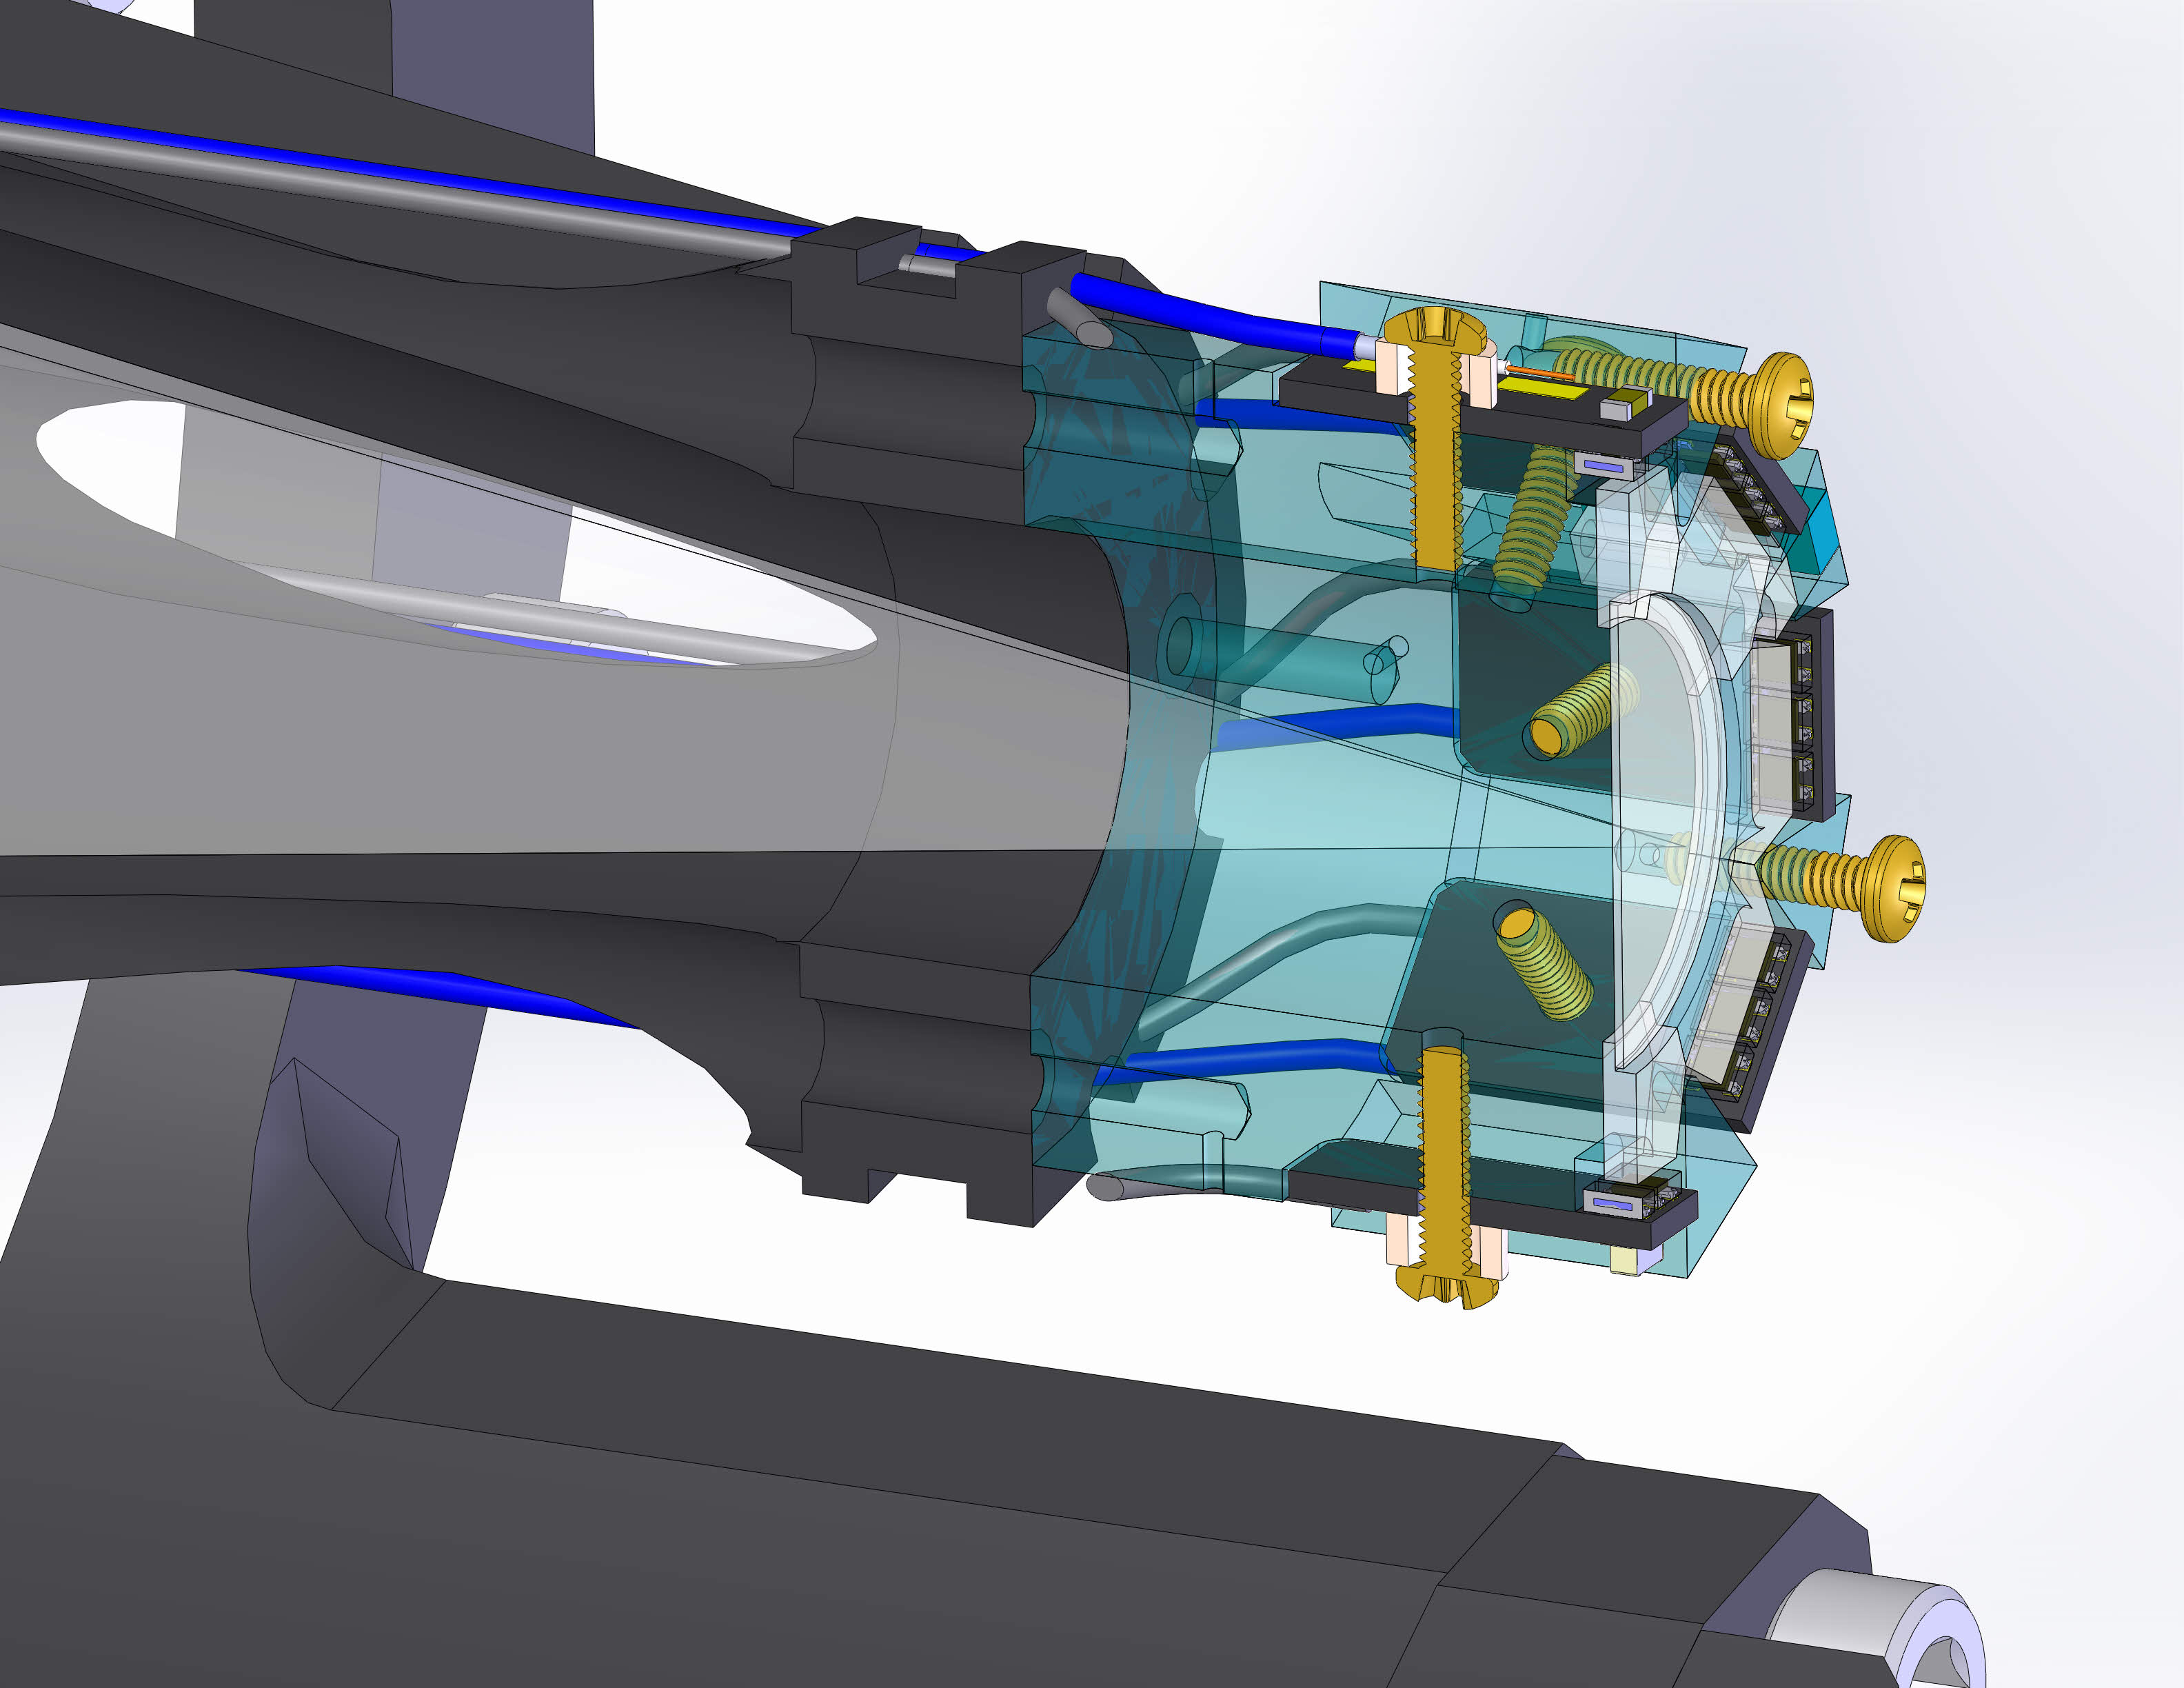
\includegraphics[width = 7cm]{sl2}
                \caption{}
                
        \end{subfigure}
        
       

        \caption{Displays the Solidworks renderings of the mini spectrometer constructed and tested on the beam line. (b) displays a magnified view of muon counter}
        \label{spect}
\end{figure}

\subsection{Setup}
The spectrometer was place on the b-leg end of the m-20 beamline, which has a beam tuned to given roughly 1000-5000 muons per second. The mock musr experiment was setup using the VME/Midas equipment. In addition to the internal SIPM muon counter an external fast phototube counter was placed near the face of the vacuum window for a performance comparison between the two counters, as phototubes this time are standard. The internal muon counter contain 8 cards with 3x1mm pixels arranged around the 0.25mm thick scintillator seen in figure \ref{spect}. Each array signal from the internal muon counter is fed into a pre-amplifier before being summed into a single channel. This signal is used as the trigger and reference start for the experiment. The 1/8 of the positron counter contains 2 4x6mm arrays on either end of the scintillator. Each pixel signal is amplified then summed and sent into a CFD which generates a stop pulse. Each end is timed independently relative to the muon counter as an up or downstream stop. In one case the two were average and provided a single stop. A piece of silver foil provided as a test sample and was centered on the positron counter. The CFD method without correction was used in this test. Leonids method was attempted however noise levels prevented feasible test.
\subsection{Results}
When a muon passes through the muon counter a start pulse is sent to the TDC. The experiment will then wait for a signal from the decaying positron. A spectrum of positrons will be observed when logging over long periods. The "rise" or "leading edge" of this spectrum gives information about the resolution of the mini spectrometer. Data was collected using both the internal and external counter as a reference for each event as displayed in figure \ref{result} and figure \ref{result2} respectively.
\begin{figure}[H]
\centering
\includegraphics[width=1.10\linewidth]{result1}
\caption{A mock musr test using internal counter. (top) Upstream Counter (middle) Downstream Counter, (bottom) up and down averaged }
\label{result}
\end{figure}

\begin{figure}[H]
\centering
\includegraphics[width=1.10\linewidth]{result2}
\caption{A mock musr test using external counter. (top) Upstream Counter (middle) Downstream Counter, (bottom) up and down averaged}
\label{result2}
\end{figure}

\subsection{Conclusions}
The best resolution measured using the internal counter was found to be 868ps, while the external counter was found to be 667ps. This test confirms the SiPM spectrometer is making progress in attaining a comparable resolution to current photo-tube detectors. However these numbers fall short of what is theoretically possible. Given the intrinsic resolution of the devices a much sharper resolution was expected. There where however a number of things that were suspected to be the cause of the poor timing. The signal provided by the SiPMs proved to be stronger than initially predicted, this led to preamp saturation at higher biasing levels. Therefore in order to prevent signal distortion device biasing was set 0.5V above breakdown. A new higher speed lower gain amplifier as well as changes to improve noise levels are recommended to improve spectrometer timing. Improved noise levels in the future could make Leonids method feasible for beamline testing which should be investigated to ensure CDF method is still favorable.
\appendix
\section{Appendix} \label{App:Appendix}
\subsection{Laser Control Program}
\begin{lstlisting}
/*compile with the command: g++ LaserControl.cxx rs232.c -Wall -Wextra -o2 -o Go
execute with ./Go -d 22.56
extra place values will be rounded ie 22.5555 = 22.56
**************************************************/
#include <iostream>
#include <stdlib.h>
#include <stdio.h>
#include <unistd.h>
#include "rs232.h"
#include <string>
#include <fstream>
#include <vector>
#include <algorithm>
#include <sstream>
#include "ctime"
#include <sys/socket.h> // Needed for the socket functions
#include <netdb.h>      // Needed for the socket functions
#include <unistd.h>  
#include <istream>
#include <cstring>
#include <alloca.h>

using namespace std;

int main(int argc, char* argv[])
{
string value;
//collect arguments
for (int i = 1; i < argc; ++i) 
{
    string arg = argv[i];
    if (arg == "-d") 
	{
        	if (i + 1 < argc)
		{ 
                value = argv[(i+1)]; 
        	} 
	    else 
		{ 
                cerr << "-option requires one argument." << std::endl;
                return 0;
        }  
    }
}

  int i=0,
      cport_nr=16,        /* /dev/ttyusb0*///see rs232.c for index
      bdrate=9600;      /* 9600 baud */

  char mode[]={'8','N','1',0},
       str[2][512];
       const char * c;
       string lasdb;
       lasdb = "A";  	
       lasdb.append(value);
       lasdb.append("\r");
       c = lasdb.c_str();  //string to const char* 
	   strcpy(str[0], c);

	  if(RS232_OpenComport(cport_nr, bdrate, mode))
	  {
	    printf("Can not open comport\n");
	    return(0);
	  }

	    RS232_cputs(cport_nr, str[i]);
	    printf("sent: %s\n", str[i]);
	    //allow attenuator to reach correct state before continuing
	    usleep(2000000);
  return(1);
}

\end{lstlisting}


\begin{thebibliography}{99} % Beamer does not support BibTeX so references must be inserted manually as below
\bibitem[Garcia, 2014]{picfsk} Lawrence Garcia (2014)
\newblock Umbilical Tests and Detector Data Analysis


\bibitem[Maneira, 2013]{p1} Jose Maneira, Rui Alves (2013)
\newblock URM design for SNO+, LIP-Coimbra

\end{thebibliography}


%%% End document
\end{document}